\lohead{Perl Nicolas}
\chapter{Elektronik}

%/\-/\-/\-/\-/\-/\-/\-/\-/\-/\-/\-/\-/\-/\-/\-/\-/\-/\-/\-/\-/\-/\-/\-/\-/\-/\-/\-/\-/\-/\-/\-/\-/\-/\-/\-/\-/\-/\-/\-/\-/\-/\-/\-/\-/\-/\-/\-/\-/\-/\-/\-/\-/\-/\-/\-/\-/\-/\-/\-/\

\section{Anforderungen}

Der elektrische Teil dieser Diplomarbeit umfasst das Entwerfen und Entwickeln eines Schaltplans und einer dazugehörigen Leiterplatte sowie das Layouten dieser und deren Bestückung.
Die Platine, gesteuert vom Mikroprozessor Atmega324P, hat die Aufgabe drei kapazitive Sensoren einzulesen, zwei Hubmagneten anzusteuern, einen Endschalter einzulesen und einen Schrittmotor anzusteuern.
Zudem hat sie die Aufgabe, jegliche elektrische Bauteile des Automaten mit Spannung zu versorgen.
Außerdem soll der Mikroprozessor dazu im Stande sein, Befehle von einem Raspberry Pi 3B+ über UART zu erhalten.
Die Möglichkeit, Debugging über eine zweite UART – Schnittstelle via Mini USB zu betreiben, soll ebenfalls gegeben sein.

\subsection{Zeitplan}

\begin{figure}[hbt!]
    \centering
    \scalebox{0.6}{
    \begin{ganttchart}[
    hgrid style/.style={black, dotted},
    calendar week text={\currentweek},
    vgrid={*6{white},*1{black,dotted}},
    x unit=1mm,
    group label font= \Large,
    y unit chart=9mm,
    y unit title=12mm,
    time slot format=isodate,
    time slot unit=year
    link/.style={->, thick}
    ]{2019-09-2}{2020-03-15}
    \gantttitlecalendar{year, month=name, week}\\

    \ganttgroup[group/.append style={draw=none}]
    {Konzeptionierung}{2019-09-02}{2019-11-31}\\ [grid]
    \ganttbar[]{Schaltungsentwürfe}{2019-09-30}{2019-11-31}\\ [grid]
    \ganttbar[]{Steckbrettaufbauten}{2019-10-14}{2019-11-31}\\ [grid]
    \ganttnewline[thick, black]

    \ganttgroup[group/.append style={draw=none}]
    {Leiterplattenherstellung}{2019-10-14}{2020-01-31}\\ [grid]
    \ganttbar[]
    {Schaltplanerstellung}{2019-10-14}{2019-12-15}\\ [grid]
    \ganttbar[]
    {Layouterstellung}{2019-11-15}{2020-01-12}\\ [grid]
    \ganttbar[]
    {Leiterplattenherstellung}{2020-01-13}{2020-01-31}\\ [grid]
    \ganttnewline[thick, black]

    \ganttgroup[group/.append style={draw=none}]
    {Prototyping}{2020-02-01}{2020-02-15}\\ [grid]
    \ganttbar[]
    {Leiterplattenfunktionsprüfungen}{2020-02-01}{2020-02-07}\\ [grid]
    \ganttbar[]
    {Gesamtsystemtests}{2020-02-01}{2020-02-15}\\ [grid]
    \ganttnewline[thick, black]

    \ganttgroup[]
    {Dokumentation}{2019-11-15}{2020-02-31}\\ [grid]

    \end{ganttchart}
    }
    \caption{Zeitplan Bereich Elektronik}
\end{figure}

\newpage

%/\-/\-/\-/\-/\-/\-/\-/\-/\-/\-/\-/\-/\-/\-/\-/\-/\-/\-/\-/\-/\-/\-/\-/\-/\-/\-/\-/\-/\-/\-/\-/\-/\-/\-/\-/\-/\-/\-/\-/\-/\-/\-/\-/\-/\-/\-/\-/\-/\-/\-/\-/\-/\-/\-/\-/\-/\-/\-/\-/\

\section{Variantenvergleiche und Konzeptionierungen}
\subsection{Mikrocontroller}
Da unser finales Konzept Einiges an Logikansteuerungen benötigt, ist es sinnvoll die Ansteuerung der Peripherie auf einen Mikrocontroller auszulagern.
Wir stellten die Anforderungen einer doppelt vorhandenen UART Schnittstelle, eine zur Kommunikation mit dem Raspberry Pi und eine, welche als Debugging-Schnittstelle genutzt werden sollte.
Außerdem schien es uns sinnvoll, einen Mikroprozessor der Atmega-Familie auszuwählen, da mit dieser bereits Erfahrung gesammelt wurde.
\subsubsection{ATmega162}
Dieser Mikrochip besitzt einen Flash-Speicher von 16kiB, einen SRAM in einer Größe von 1kiB und einen E²PROM-Speicher von 512 Bytes.
Der ATmega162 verfügt über eine SPI und zwei UART Schnittstellen sowie 35 I/O Register und zwei Timer.
Er kann mit einer Gleichspannung von 2.7V bis 5.5V betrieben werden.
\subsubsection{ATmega324P}
Der ATmega324P ist ein Mikrochip, welcher 32kiB an Flash-Speicher, 1kiB an E²PROM-Speicher sowie 1kiB an SRAM mit sich bringt.
Er verfügt über 32 I/O Register, eine SPI Schnittstelle, eine I²C Schnittstelle, zwei UART Schnittstellen sowie drei flexible Timer.
Außerdem lässt er sich mit einer Gleichspannung von 1.8V bis 5V betreiben.
\subsubsection{ATmega128}
Der ATmega128 besitzt einen E²PROM-Speicher von 4kiB, einen 123kiB großen Flash-Speicher und einen SRAM von 4kiB .
Er besitzt zwei UART-, eine SPI- sowie eine I²C-Schnittstelle.
Zusätzlich bietet er vier Timer und 53 I/O Pins.
Er kann mit einer Gleichspannung von 4.5V bis 5.5V betrieben werden.
\subsubsection{Mikrocontroller-Auswahl}

\begin{table}[h]
\centering
\begin{tabular}{|
>{\columncolor[HTML]{FFFFFF}}l |
>{\columncolor[HTML]{FFFFFF}}l |
>{\columncolor[HTML]{FFFFFF}}l |
>{\columncolor[HTML]{FFFFFF}}l |
>{\columncolor[HTML]{FFFFFF}}l |}
\hline
& \textbf{ATmega162} & \textbf{ATmega324P} & \textbf{ATmega128} \\ \hline
Preis & gering & gering & mittel            \\ \hline
Flash-Speicher & 16kiB & 32kiB & 128kiB     \\ \hline
EEPROM-Speicher & 512B & 1kiB & 4kiB        \\ \hline
I/O-Pins & 35 & 32 & 53                     \\ \hline
UART-Schnittstellen & 2 & 2 & 2             \\ \hline
SPI-Schnittstelle & ja & ja & ja            \\ \hline
Versorgungsspannung & 2,7V-5V & 1,8V-5V & 4,5V-5V  \\ \hline
\end{tabular}
\caption{Vergleich der Mikrocontrollerattribute}
\end{table}

Unsere Entscheidung fiel auf den ATmega324P, da dieser die nötigen Parameter, wie eine Versorgungsmöglichkeit mit 3,3V und einen ausreichend großen, programmierbaren Speicher, mit sich bringt.

\subsection{Schrittmotor-Ansteuerung}
Um jenen, im Automaten verbauten, Schrittmotor ansteuern zu können, ist eine Baugruppe von Nöten.
Für das Ansteuern von Schrittmotoren gibt es verschiedenste Möglichkeiten.
In den folgenden Unterkapiteln werden einzelne genannt, ein Variantenvergleich durchgeführt und sich für eine Variante entschieden.

\subsubsection{DIY-H-Brücke}

Mithilfe einer sogenannten H-Brücke ist es möglich, Schrittmotoren mitunter der Verwendung eines Mikrocontrollers anzusteuern.
Der von uns ausgewählte Schrittmotor 12HS19-2004S1 ist bipolarer Art und weißt 2 Spulen auf, weshalb er sich von zwei H-Brücke steuern lässt.
Für das Ansteuern einer H-Brücke werden drei Steuersignale benötigt:
zwei digitale Signale sowie ein PWM-Signal.

\begin{figure}[ht]
\centering
\begin{circuitikz}[european, scale = 1]
\draw (3,0) to [short, -*](5,0) to (7,0);
\draw (2,2) to (2.5,2);
\draw (3,2)node[npn, bodydiode]{};
\draw (3,5)node[pnp, bodydiode]{};
\draw (7,2.5) to (7,4.5);
\draw (3,2.5) to (3,4.5);
\draw (3,5.5) to (3,6) to [short, -*](5,6) to (7,6) to (7, 5.5);
\draw (5,6)node[vcc]{Vcc};
\draw (3,3.5) to [short,*-o](4,3.5);
\draw (7,3.5) to [short,*-o](6,3.5);
\draw (7,2)node[npn, bodydiode, xscale = -1]{};
\draw (7,5)node[pnp, bodydiode,xscale = -1]{};
\draw (0.5,5) to [R, l=$R_1$, o-](2,5) to (2.5,5);
\draw (9.5,5) to [R, l_=$R_2$, o-](8,5) to (7.5,5);
\draw (0.5,2) to [R, l=$R_3$](2,2) to (2.5,2);
\draw (9.5,2) to [R, l_=$R_4$](8,2) to (7.5,2);
\draw (9.5,2)node[american and port, xscale = -1](){};
\draw (0.5,2)node[american and port](){};
\draw (-0.9,1.725) to [short, o-](-0.9,1.725);
\draw (-0.9,2.275) to [short, o-](-0.9,2.275);
\draw (10.9,1.725) to [short, o-](10.9,1.725);
\draw (10.9,2.275) to [short, o-](10.9,2.275);
\draw (5,4.3)node[anchor=north]{Spule 1};
\draw (-1,1.7)node[anchor=east]{PWM-Signal};
\draw (-1,2.3)node[anchor=east]{Steuersignal};
\draw (13.3,2.3)node[anchor=east]{Steuersignal};
\draw (13.5,1.7)node[anchor=east]{PWM-Signal};
\draw (0.5,5)node[anchor=east]{Steuersignal};
\draw (12,5)node[anchor=east]{Steuersignal};
\draw (3,1.5) to (3,0);
\draw (7,1.5) to (7,0);
\draw (3,0) to (5,0) node[rground]{};
\end{circuitikz}
\caption{Aufbau einer H-Brücke}
\end{figure}

Grundsätzlich ist zu sagen, dass eine H-Brücke aus vier Transistoren und vier Schutzdioden besteht. \\
Ein konkreter Aufbau einer H-Brücke kann der Abbildung 2.1 entnommen werden.
Bei dieser Variante einer H-Brücke sind zwei NPN-Transistoren und zwei PNP-Transistoren vorhanden, von denen jeder einen Basisvorwiderstand besitzt.
Wie in Abbildung 2.1 zu erkennen ist, befindet sich vor jedem Basiswiderstand der NPN-Transistoren ein UND-Gatter, mit dem jeweils ein digitales Steuersignal und das PWM-Signal zusammengeführt werden.
Zusätzlich befindet sich parallel zu jedem Bipolartransistor eine Schutzdiode.
Diese haben folgende Aufgabe:\\\\
Ein Nebeneffekt der Funktionsweise eines Motors, ist die Erzeugung von Energie.
Bei einem Deaktivieren der Transistoren, um den Motor zu stoppen, muss diese erzeugte Energie des Motors auf irgendeine Weise freigesetzt werden können.
Um ein Beschädigen der Transistoren zu vermeiden, verwendet man diese Dioden, um dem Strom einen Pfad zu bieten, der die Energie freisetzt. \\\\



\begin{figure}[ht]
\centering
\begin{circuitikz}[european, scale = 0.9]

% Mikrocontroller
\draw [line width=1.5pt](-7,4) -- (-3,4) -- (-3,11) -- (-7,11) -- (-7,4);
\draw (-5,8)node[anchor=north]{ATmega324P};
\draw (-5,4.6)node[anchor=north]{OC1A};
\draw (-5,11)node[anchor=north]{OC1B};
\draw (-6.5,4.6)node[anchor=north]{PD2};
\draw (-3.5,4.6)node[anchor=north]{PD3};
\draw (-6.5,11)node[anchor=north]{PD0};
\draw (-3.5,11)node[anchor=north]{PD1};


% 1. Spulenanschluss
\draw (3,8) to [short, -*](5,8) to (7,8);
\draw (2,10) to (2.5,10);
\draw (3,10)node[npn, bodydiode]{};
\draw (3,13)node[pnp, bodydiode]{};
\draw (7,10.5) to (7,12.5);
\draw (3,10.5) to (3,12.5);
\draw (3,13.5) to (3,14) to [short, -*](5,14) to (7,14) to (7, 13.5);
\draw (5,14)node[vcc]{Vcc};
\draw (3,11.5) to [short,*-o](4,11.5);
\draw (7,11.5) to [short,*-o](6,11.5);
\draw (7,10)node[npn, bodydiode, xscale = -1]{};
\draw (7,13)node[pnp, bodydiode,xscale = -1]{};

\draw (0.5,13) to [R, l=$R_1$, ](2,13) to (2.5,13);
\draw (9.5,13) to [R, l_=$R_2$, ](8,13) to (7.5,13);
\draw (9.5,13)to [short,-*](13,13);
\draw (0.5,10) to [R, l=$R_3$](2,10) to (2.5,10);
\draw (9.5,10) to [R, l_=$R_4$](8,10) to (7.5,10);

\draw (9.5,10)node[american and port, xscale = -1](){};
\draw (0.5,10)node[american and port](){};

\draw (-0.9,9.69) to (-2.5,9.69) to [short,-*](-2.5,16);
\draw (-0.9,10.31) to (-2,10.31) to (-2,13) to (0.5,13);
\draw (-2,13) to [short,*-](-4,13) to (-4,11);
\draw (10.9,9.69) to (13,9.69) to (13,17) to (-6,17) to (-6,11);
\draw (10.9,10.31) to (12,10.31) to (12,13) to (12,16) to (-5,16) to (-5,11);

\draw (3,13.7)node[anchor=east]{Q1};
\draw (7,13.7)node[anchor=west]{Q2};
\draw (3,10.7)node[anchor=east]{Q3};
\draw (7,10.7)node[anchor=west]{Q4};

\draw (-0.5,11.2)node[anchor=north]{IC1};
\draw (10,11.2)node[anchor=north]{IC2};

\draw (5,12.3)node[anchor=north]{Spule 1};
\draw (3,9.5) to (3,8);
\draw (7,9.5) to (7,8);
\draw (3,8) to (5,8) node[rground]{};

% 2. Spuelanschluss
\draw (3,0) to [short, -*](5,0) to (7,0);
\draw (2,2) to (2.5,2);
\draw (3,2)node[npn, bodydiode]{};
\draw (3,5)node[pnp, bodydiode]{};
\draw (7,2.5) to (7,4.5);
\draw (3,2.5) to (3,4.5);
\draw (3,5.5) to (3,6) to [short, -*](5,6) to (7,6) to (7, 5.5);
\draw (5,6)node[vcc]{Vcc};
\draw (3,3.5) to [short,*-o](4,3.5);
\draw (7,3.5) to [short,*-o](6,3.5);
\draw (7,2)node[npn, bodydiode, xscale = -1]{};
\draw (7,5)node[pnp, bodydiode,xscale = -1]{};

\draw (0.5,5) to [R, l=$R_5$, ](2,5) to (2.5,5);
\draw (9.5,5) to [R, l_=$R_6$, ](8,5) to (7.5,5);
\draw (0.5,2) to [R, l=$R_7$](2,2) to (2.5,2);
\draw (9.5,2) to [R, l_=$R_8$](8,2) to (7.5,2);

\draw (9.5,2)node[american and port, xscale = -1](){};
\draw (0.5,2)node[american and port](){};

\draw (-0.9,1.685) to [short, -*](-5,1.685);
\draw (-0.9,2.315) to [short,-*](-2,2.315) to (-2,5) to (0.5,5);
\draw (-0.9,2.315) to (-4,2.315) to (-4,4);
\draw (10.9,1.685) to (12,1.685);
\draw (10.9,2.315) to (12,2.315) to (12,5) to (9.5,5);
\draw (12,1.685) to (12,-1) to (-5,-1) to (-5,4);
\draw (12,5) to [short,*-](13,5) to (13,-2) to (-6,-2) to (-6,4);

\draw (-0.5,3.2)node[anchor=north]{IC3};
\draw (10,3.2)node[anchor=north]{IC4};

\draw (3,5.7)node[anchor=east]{Q5};
\draw (7,5.7)node[anchor=west]{Q6};
\draw (3,2.7)node[anchor=east]{Q7};
\draw (7,2.7)node[anchor=west]{Q8};

\draw (5,4.3)node[anchor=north]{Spule 2};
\draw (3,1.5) to (3,0);
\draw (7,1.5) to (7,0);
\draw (3,0) to (5,0) node[rground]{};

\end{circuitikz}
\caption{Anschluss einer H-Brücke an einen Mikrocontroller}
\end{figure}

In der obigen Abbildung 2.2 wird eine konkrete Verbindung von zwei H-Brücken in Kombination mit einem Mikrocontroller dargestellt.
Da sich die Ansteuerung der beiden H-Brücken gleich gestaltet, wird zur vereinfachten Funktionserklärung nur die obere behandelt. \\
Mithilfe des Timer 0 wird am Ausgang OC1B des Mikrocontrollers ein PWM-Signal erzeugt, mithilfe dessen, abhängig vom gewählten Duty-Cycle, Spannungssignale in gewissen Zeitabständen geschickt werden.
Dadurch befindet sich jeweils an einem Eingang des UND-Gatters mit der Bezeichnung IC1 und an einem Eingang des UND-Gatters mit der Bezeichnung IC2 ein Signal mit einem HIGH-Pegel (Spannung) oder
LOW-Pegel (keine Spannung). \\\\
Je nach gewollter Drehrichtung, ist der Motor über die Transistoren anders anzusteuern: \\
Um den Schrittmotor nach Rechts drehen zu lassen, muss am Ausgang PD0 ein HIGH-Signal erzeugt werden.
Am Ausgang PD1 muss ein LOW-Signal erzeugt werden, da ansonsten der PNP-Transistor Q1 sperrt und kein Stromfluss gewährleistet wäre.
Durch das HIGH-Signal, ausgehend vom Ausgang OC1B, befindet sich ein HIGH-Signal am unteren Eingang des UND-Gatters IC2.
Wenn nun ein HIGH-Pegel ausgehend vom Ausgang PD0 kommt, liefert das UND-Gatter IC2 ein HIGH-Signal weiter an den NPN-Transistor Q4, welcher somit leitend wird und den Stromkreis schließt. \\\\
Um den Schrittmotor nach Links drehen zu lassen, wird am Ausgang PD1 ein HIGH-Signal gesetzt.
Am Ausgang PD0 muss ein LOW-Signal erzeugt werden, da ansonsten der PNP-Transistor Y sperrt und kein Stromfluss gewährleistet wäre.
Durch das HIGH-Signal, ausgehend vom Ausgang PD1, befindet sich ebenfalls ein HIGH-Signal am oberen Eingang des UND-Gatters.
Wenn nun ein HIGH-Pegel vom Ausgang OC1B bereitgestellt wird, liefert das UND-Gatter IC1 ein HIGH-Signal weiter an den NPN-Transistor Q3, welcher somit leitend wird und
ein Fließen des Stromes durch die Motorwicklung bewirkt.

\begin{itemize}
\item \textbf{Vorteile}
\begin{itemize}
\item günstig
\end{itemize}
\item \textbf{Nachteile}
\begin{itemize}
\item viele Bauteile
\item Bauteile müssen erst dimensioniert werden
\item Kosten könnten sich aufgrund hoher Verlustleistung durch einen Kühlkörper erhöhen
\end{itemize}
\end{itemize}

\subsubsection{Schrittmotor-Treibermodule}
Schrittmotor-Treiber sind Module, welche mithilfe von externen Signalen in der Lage sind, Schrittmotoren steuern zu können.

\begin{itemize}
\item \textbf{Vorteile}
\begin{itemize}
\item platzsparend
\item leicht austauschbar
\item leicht verwendbar
\end{itemize}
\item \textbf{Nachteile}
\begin{itemize}
\item Kosten könnten sich, aufgrund eines Kühlkörpers erhöhen
\end{itemize}
\end{itemize}

\subsubsection{A4988}
Das Modul kann mit einer Eingangsspannung von 8V bis 35V arbeiten und kann ohne den Einsatz eines Kühlkörpers bis zu 1A pro Phase liefern.
Der Treiber ist jedoch darauf ausgelegt, einen Strom von 2A mit zusätzlicher Kühlung zur Verfügung stellen zu können.
Es besteht kein Bedarf daran Phasenfolgetabellen, Hochfrequenz-Steuerleitungen oder komplexe Schnittstellen zu programmieren.
Das A4988 Treiber-Modul von Allegro bietet viele Möglichkeiten.
Zu nennen ist die Eigenschaft einer einstellbaren Begrenzung des abgegebenen Stroms über ein Potentiometer.
Dadurch können Spannungen über der Nennspannung des Schrittmotors verwendet werden, um höhere Schrittgeschwindigkeiten zu erreichen.
Zusätzlich wird die Gewährleistung eines Überstromschutz und Übertemperaturschutzes sowie eine Überspannungsabschaltung versichert.
Erdschluss- und Kurzschlussschutz sind ebenfalls gegeben.
Der Schrittmotortreiber bietet fünf verschiedene Mikroschrittauflösungen: Voll-, Halb-, Viertel-, Achtel- und Sechzehntel-Schrittmodus.

\subsubsection{DRV8825}
Diesem Treiber-Board von Texas Instruments ist es Möglich mit einer Spannung von 8,2 V bis 45 V zu arbeiten.
Er kann ohne eine bestimmte Kühlung bis zu 1,5 A pro Phase liefern.
Ausgelegt ist dieses Modul auf einen Strom von 2,5A, welche mit zugeführter Kühlung auch getrieben werden können.
Der DRV8825 arbeitet mit einem Logikpegel von 3,3V bis 5V und bietet die Möglichkeit einer einstellbaren Strombegrenzung.
Das Modul besitzt ebenfalls die Eigenschaften eines Überstrom- und Übertemperaturschutzes sowie sechs Mikroschrittauflösungen, welche bis zu einer Zweiunddreißigstel-Auflösung reichen.
Die Besonderheit eines SLEEP-MODE mit geringen Stromverbrauch und eines eingebauten Unterspannungsschutzes sind zusätzlich gegeben.
Der DRV8825-Treiber verfügt über eine Schnittstelle und eine Pinbelegung, welche beinahe mit denen des A4988-Schrittmotortreibers identisch sind,
sodass er in vielen Anwendungen als leistungsstärkerer Ersatz verwendet werden kann.

\subsubsection{TB6600}
Dieser Ein-Achsen-Schrittmotortreiber ist für Hybride Schrittmotoren mit 2 oder 4 Phasen geeignet.
Der TB6600 arbeitet mit einer Spannung von 9V bis 40V und ist für einen Ausgangsstrom von 0,7A bis 4A ausgelegt.
Das Modul bringt die Eigenschaften eines Übersitzungs-, Kurzschluss- und Überstromschutzes sowie einen großflächigen Kühlkörper mit sich.
Der Ausgangsstrom ist mittels DIP-Schalter in acht Schritten wählbar.
Sechs verschieden wählbare Mikroschrittauflösungen, welche bis zu einer Auflösung von Zweiunddreißigstel reichen, werden zur Verfügung gestellt.
Die Kontrolllogik dieses Treibers umfasst eine Spannung von 5V. Das Gewicht von
200dag und eine Größe von 57mm x 96mm x 28mm unterscheiden sich wesentlich von den anderen Treibermodulen.

\subsubsection{Treiber-Auswahl}

\begin{table}[h]
\centering
\begin{tabular}{|
>{\columncolor[HTML]{FFFFFF}}l |
>{\columncolor[HTML]{FFFFFF}}l |
>{\columncolor[HTML]{FFFFFF}}l |
>{\columncolor[HTML]{FFFFFF}}l |
>{\columncolor[HTML]{FFFFFF}}l |}
\hline
& \textbf{A4988} & \textbf{DRV8825} & \textbf{TB6600} \\ \hline
Preis & gering & gering & mittel    \\ \hline
Max.Strom & 2A & 2.2A & 4A    \\ \hline
Spannungsbereich & 8V-35V & 8.2V-35V & 9V-40V      \\ \hline
Logik-Pegel & 3.3V-5V & 3.3V-5V & 5V        \\ \hline
Max.Schrittauflösung & 16 & 32 & 32        \\ \hline
Größe & klein & klein & groß        \\ \hline
\end{tabular}
\caption{Vergleich der Treibermodule}
\end{table}

Da unsere Wahl auf den Schrittmotor 12HS19-2004S1 gefallen ist, wäre es ratsam einen Treiber auszuwählen, welcher 2A Strom zur Verfügung stellen kann.
Unsere Treiber-Auswahl ist somit auf den DRV8825 gefallen, da dieser alle erforderlichen Kriterien, wie einen geringen Preis und den 3,3V Logikpegel, erfüllt und ein gutes Allroundpaket mit sich bringt.
Ein Begründung, warum die Wahl auf das DRV8825 Modul und nicht das A4988 Modul fiel, sind die größere Spannungsbandbreite, der höhere maximale Strom pro Phase sowie die höhere maximale Schrittauflösung.

\subsection{Detektion der Kartenposition}

\subsubsection{Kapazitive Sensoren}
Die Funktion von kapazitiven Sensoren ist mit der eines offenen Kondensators zu vergleichen.
Zwischen der Messelektrode und der GND - Elektrode bildet sich ein elektrisches Feld.
Dringt ein Material mit einer Dielektrizitätszahl $\varepsilonup$r größer als Luft in das elektrische Feld ein, so vergrößert sich je nach dieser Zahl des Material die Kapazität des Feldes.
Es wird zwischen zwei Arten von kapazitiven Sensoren unterschieden: \\\\

\textbf{Sensoren mit GND-Elektrode} \\
Ein bündiger Einbau dieser Sensoren ist möglich, da sich ihr Messfeld von der Messelektrode zur integrierten GND-Elektrode ausbreitet.
Diese Variante dient sich gut zur Detektion von nicht leitenden Materialien. \\\\

\textbf{Sensoren ohne GND-Elektrode} \\
Ein bündiges Einbauen dieser Art ist nicht vorteilhaft.
Eine integrierte GND-Elektrode ist nicht vorhanden, sie wird nämlich vom zu konstatierenden Objekt dargestellt.
Diese Bauform weist eine geringe Empfindlichkeit gegen Verschmutzung auf.
Für hohe Schaltabstände sind leitende und geerdete Gegenstände von Vorteil.

\subsubsection{Ultraschall-Sensoren}
Die meisten Ultraschall-Sensoren arbeiten nach dem Prinzip der Laufzeitmessung von hochfrequenten Schallimpulsen.
Ein Sensor sendet zyklisch einen kurzen, hochfrequenten Schallimpuls aus, welcher sich in der Luft fortpflanzt und am getroffenen Gegenstand reflektiert wird.
Das Echo wird vom Sensor wieder aufgenommen und aus der Zeitspanne zwischen dem Zeitpunkt des Absendens und dem Zeitpunkt des Erfassens wir der Abstand vom Sensor berechnet.
So ist es diesem Art von Sensor möglich, unterschiedlichste Materialien wie Metall oder Holz aufzufassen.
Lediglich schalldämpfende Materialien können nur schwer erfasst werden.
Diese Art von Sensoren ist in der Lage berührungslos Objekte zu erkennen und ihre Entfernung zum Sensor zu messen.
Ein fast wartungsfreier Betrieb ist möglich.

\subsubsection{Optische Sensoren}
Ein optischer Sensor sendet über seine eigene Lichtquelle einen Lichtstrahl aus.
Zu unterscheiden sind hierbei Lichtschranken und Reflexionstypen.

\begin{itemize}
\item Optische Sensoren des Lichtschrankentyps detektieren Unterbrechungen einer Lichtachse, welche durch ein Zielobjekt hervorgerufen werden.
\item Lichtsender und Empfänger sind baulich getrennt.

\item Sensoren des Reflexionstyps werden zur Erfassung eines vom Zielobjekt reflektierten Lichtstrahls eingesetzt.
\end{itemize}

Optische Sensoren besitzen eine fast wartungsfreie, langfristigen Betrieb, da die Detektion kontaktlos erfolgt.
Diese Art von Sensoren kann für nahezu jedes beliebige Material eingesetzt werden.
Es sind große Erkennungsabstände möglich.

\subsubsection{Sensoren-Auswahl}

\begin{table}[h]
\centering
\begin{tabular}{|
>{\columncolor[HTML]{FFFFFF}}l |
>{\columncolor[HTML]{FFFFFF}}l |
>{\columncolor[HTML]{FFFFFF}}l |
>{\columncolor[HTML]{FFFFFF}}l |
>{\columncolor[HTML]{FFFFFF}}l |}
\hline
& \textbf{Kapazitive Sensoren} & \textbf{Ultraschall-Sensoren} & \textbf{Optische Sensoren} \\ \hline
Preis & gering & hoch & mittel    \\ \hline
Platzbedarf & gering & gering & mittel   \\ \hline
Genauigkeit & hoch & mittel & hoch        \\ \hline
\end{tabular}
\caption{Vergleich der Sensorattribute}
\end{table}

Unsere Wahl fiel auf einen kapazitiven Sensor da dieser für uns bereits für einen erschwinglichen Preis alles Nötige mit sich bringt: einen hohen Grad an Genauigkeit sowie einen geringen Platzbedarf.
Somit fiel unsere Wahl auf den LJC18A3, welcher mit einer Versorgungspannung von 6V bis 36V arbeitet und metallische und nichtmetallische Gegenstände in einem Schaltabstand von 1 bis 10mm erfassen kann.
Dieser Sensor konnte mit einem sehr geringen Preis in unserem Besitz gebracht werden und zeigte schon bei den ersten Tests, dass er seiner Aufgabe gewachsen war.

\subsection{Erfassung der Position des Motors}
\subsubsection{Endschalter}
Diese Realisierung umfasst einen Endschalter, welcher als Referenzpunkt vor jedem Mischvorgang angefahren wird, von dem aus die benötigten Schritte aufgetragen werden.

\subsubsection{Lichtschranke}
Eine Lichtschranke würde, wie der Endschalter, am Anfang angefahren werden und so ebenfalls als Referenzpunkt fungieren.

\subsubsection{Varianten-Auswahl}
\begin{table}[h]
\centering
\begin{tabular}{|
>{\columncolor[HTML]{FFFFFF}}l |
>{\columncolor[HTML]{FFFFFF}}l |
>{\columncolor[HTML]{FFFFFF}}l |
>{\columncolor[HTML]{FFFFFF}}l |
>{\columncolor[HTML]{FFFFFF}}l |}
\hline
& \textbf{Endschalter} & \textbf{Licntschranke} \\ \hline
Preis & sehr gering & mittel  \\ \hline
Platzbedarf & sehr gering & mittel     \\ \hline
Genauigkeit & mittel & hoch     \\ \hline
\end{tabular}
\caption{Vergleich der Sensorattribute}
\end{table}

Unsere Wahl fiel auf den Endschalter, da dieser leicht in kürzester Zeit zu einem geringen Preis erworben werden konnte und ausreichend Genauigkeit mit sich bringt.

\subsection{Spannungsversorgung}
\subsubsection{Doppel-Schaltnetzteil mit zweierlei Ausgangsspannungspegeln}
Diese Variante wäre mit einem Netzteil zu realisieren, welches lediglich über einen Kaltgerätestecker mit einer Netzspannung von 230V AC in Verbindung gebracht werden müsste,
um die Versorgung der Peripherie zu gewährleisten.
Sensoren, Schrittmotor und Hubmagneten würden über den 12V DC Ausgang versorgt werden,
die Versorgung des Mikrocontrollers und des Raspberry Pi 3B+ würde über den 5V Ausgang des Schaltnetzteils realisiert werden.
Es müsste jedoch ein Pegelwandler zwischen dem Raspberry Pi und dem Mikrocontroller eingebaut werden, da die Spannungslogik des Raspberry auf 3.3V basiert und die des Mikrocontrollers auf 5V .

\subsubsection{Schaltnetzteil und Schaltregler}
Bei dieser Realisierung handelt es sich um ein mit 230V Wechselspannung versorgtes Netzteil, welches diese in ein 12V Gleichspannungssignal tranferiert.
Jene 12V werden von jeglichen Aktoren und Sensoren genutzt.
Außerdem wird mithilfe der 12V ein Schaltregler mit Spannung versorgt, welcher die 5V Spannungsversorgung des Raspberry Pi bereitstellt.
Über die GPIO Pins des Raspberry Pi wird folgend der Mikrocontroller mit 3.3V versorgt.

\subsubsection{Schaltnetzteil und Festspannungsregler}
Bei dieser Alternative wird ein Schaltnetzteil mit 230V AC versorgt, welches ein 12V DC Signal am Ausgang bereitstellt.
Dieses wird für die 12V Peripherie genutzt sowie als Versorgung für einen Festspannungsregler, welcher 12V zu 5V umwandelt.
Mit diesem Signal ist die Versorgung des Raspberry Pi bereitgestellt.
Die Versorgung des Mikrocontroller wird über zwei 3.3V GPIO Pins gewährleistet.


\subsubsection{Auswahl der Spannungsversorgung}
\begin{table}[htbp]
\centering
\begin{tabular}{|
>{\columncolor[HTML]{FFFFFF}}l |
>{\columncolor[HTML]{FFFFFF}}l |
>{\columncolor[HTML]{FFFFFF}}l |
>{\columncolor[HTML]{FFFFFF}}l |
>{\columncolor[HTML]{FFFFFF}}l |}
\hline
& \textbf{Doppel-Schaltnetzteil} & \textbf{SN und Schaltregler} & \textbf{SN und Festspannungsregler} \\ \hline
Preis & hoch & mittel & sehr gering    \\ \hline
\multicolumn{1}{|l|}{\begin{tabular}[c]{@{}l@{}}
Platzbedarf\\ und Gewicht
\end{tabular}} & \multicolumn{1}{l|}{hoch} & \multicolumn{1}{l|}{gering} & \multicolumn{1}{l|}{gering} \\ \hline
Bauteilbedarf & gering & mittel & sehr gering        \\ \hline
\end{tabular}
\caption{Vergleich der Spannungsversorgungsmodul-Attribute}
\end{table}

Unsere Wahl fiel auf die Variante des 12V Schaltnetzteils mit 5V Festspannungsregler, da diese für einen geringen Preis erhältlich ist
und einen sehr geringen Bedarf an Platz und Bauteilen mit sich bringt.

Den Mikrocontroller versorgen wir mit dem 3.3V Ausgang des Raspberry Pi 3B+.
Aufgrund der Tatsache, dass der Mikrocontroller mit einer Versorgung von 5V auch mit einer Logik von +5V arbeiten würde und somit ein Pegelwandler zu 3.3V nötig wäre,
verwarfen wir die Idee diesen mit 5V zu versorgen.

\newpage

\subsection{Blockschaltbild der gesamten Elektronik}

\begin{figure}[hb]
\centering
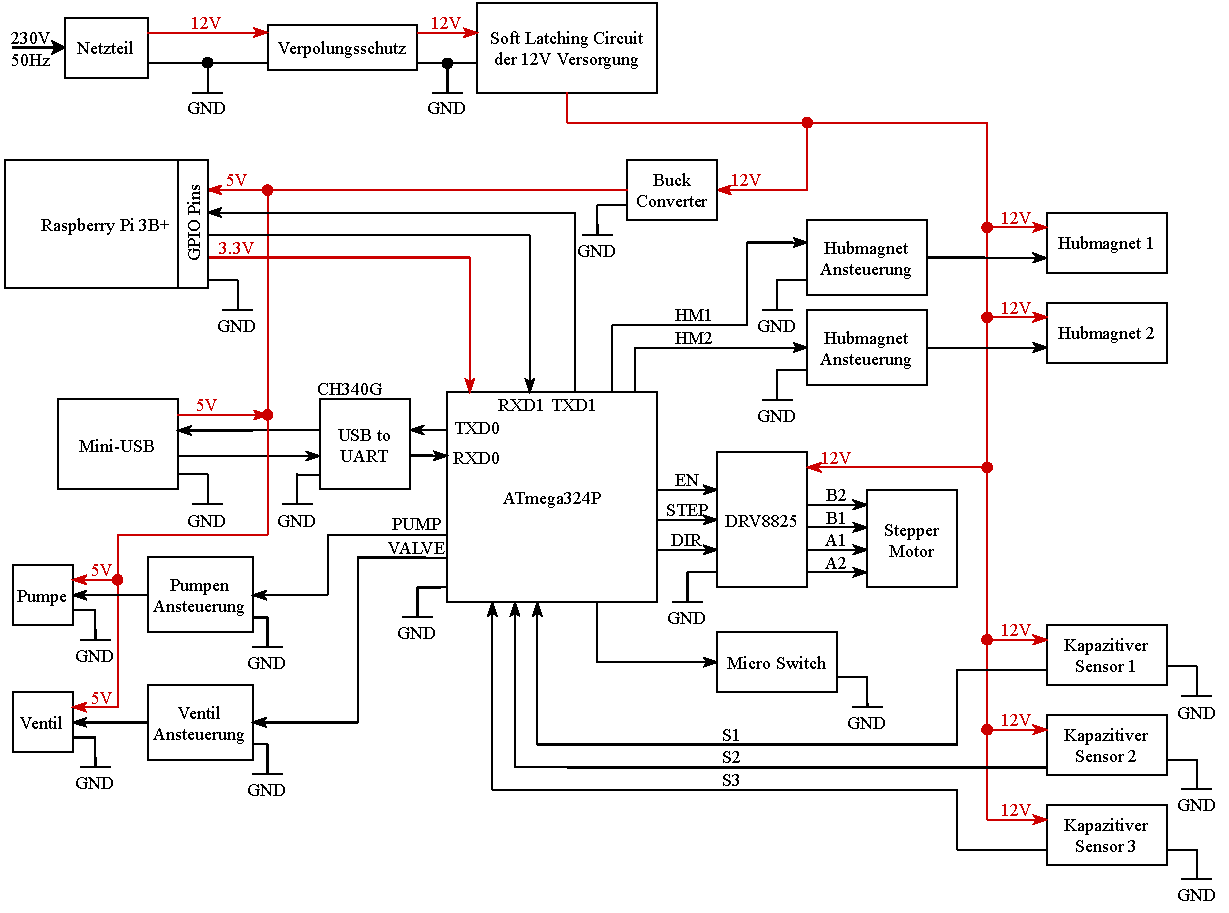
\includegraphics[scale=0.85,page=1]{fig/elektro/ElectroBlockDiagram.pdf}
\caption{Blockschaltbild der gesamten Elektronik}
\end{figure}

\newpage

%/\-/\-/\-/\-/\-/\-/\-/\-/\-/\-/\-/\-/\-/\-/\-/\-/\-/\-/\-/\-/\-/\-/\-/\-/\-/\-/\-/\-/\-/\-/\-/\-/\-/\-/\-/\-/\-/\-/\-/\-/\-/\-/\-/\-/\-/\-/\-/\-/\-/\-/\-/\-/\-/\-/\-/\-/\-/\-/\-/\

\section{Schaltplan}

\subsection{Verpolungsschutz}

Da die Versorgungsspannung der elektrischen Baugruppen über eine Klemme eingespeist wird und eine Verwechslung der Anschlusspolaritäten nicht unwahrscheinlich ist,
vermag es einen Verpolungsschutz zu verwerden um die dahinter gelegene Elektronik zu schützen.

\subsubsection{Verpolungsschutz mit einer Diode}

Die einfachste Methode diesen Schutz zu gewährleisten, ist über eine Diode.
Jedoch bringt diese Methode einen erheblichen Nachteil von einem Spannungsabfall von bis zu 1V mit sich, was bei 12V immerhin 8.33 Prozent entsprechen.

\begin{figure}[ht]
\centering
\begin{circuitikz}[european, scale = 1.2]
\draw (0,0) node[anchor=east] {-} to [short, o-*] (3,0);
\draw (2,3) to[/tikz/circuitikz/bipoles/length=1cm, D, l=$D1$](4,3){};
\draw (1,3) to [short, -o](0,3)node[anchor=east]{+};
\draw (1,3) to [short, -o](6,3)node[anchor=west]{+};
\draw (3,0) to [short, *-o](6,0)node[anchor=west]{-};
\draw (4,0) to (3,0) node[rground]{};
\draw (0,2.8) -- node[right] {$U_\mathrm{e}$}node[sloped,currarrow,pos=1] {}(0,0.2);
\draw (6,2.8) -- node[right] {$U_\mathrm{a}$}node[sloped,currarrow,pos=1] {}(6,0.2);
\end{circuitikz}
\caption{Variante mithilfe einer Diode}
\end{figure}

\subsubsection{Verpolungsschutz mit einer Sicherung und einer Diode}

Diese Realisierung bringt die Verwendung einer Sicherung und einer Diode mit sich.

Bei verpolter anliegender Eingangsspannung brennt die Sicherung, bei ausreichendem,
von der Spannungsversorgung zur Verfügung gestelltem Strom, durch.
Jedoch entsteht die negative Tatsache einer verpolten Spannung von bis zu 1V, bis die Sicherung auslöst.

\begin{figure}[ht]
\centering
\begin{circuitikz}[european, scale = 1.2]
\draw (0,0) node[anchor=east] {-} to [short, o-*] (3,0);
\draw (1,3) to[R, l=$F1$](3,3){};
\draw (4,0) to[/tikz/circuitikz/bipoles/length=1cm, D, l=$D1$, *-*](4,3){};
\draw (1,3) to [short, -o](0,3)node[anchor=east]{+};
\draw (1,3) to [short, -o](6,3)node[anchor=west]{+};
\draw (3,0) to [short, *-o](6,0)node[anchor=west]{-};
\draw (4,0) to (3,0) node[rground]{};
\draw (4,0) to (4,2);
\draw (0,2.8) -- node[right] {$U_\mathrm{e}$}node[sloped,currarrow,pos=1] {}(0,0.2);
\draw (6,2.8) -- node[right] {$U_\mathrm{a}$}node[sloped,currarrow,pos=1] {}(6,0.2);
\end{circuitikz}
\caption{Zerstörerische Variante mithilfe einer Sicherung und einer Diode}
\end{figure}

\subsubsection{Verpolungsschutz mithilfe eines P-Kanal MOSFET}

Der P-Kanal MOSFET leitet, wenn das Gate um U\textsubscript{GSth} negativer ist als der Spannungspegel anliegend am Source.
Das Anlegen einer korrekt gepolten Spannung am Eingang des MOSFET bewirkt ein Leiten der Bulk-Diode, sodass am Sourceeingang die Eingangsspannung ankommt.
Weil die am Source anliegende Spannung weitaus positiver als U\textsubscript{GSth} ist, leitet der MOSFET .
Die eingebaute Z-Diode begrenzt U\textsubscript{GS} auf einen für den MOSFET ungefährilichen Wert.
Die Tatsache, dass der MOSFET quasi verkehrt herum leitet und der Drain somit positiver als der Source ist, gilt als redondant, da es sich lediglich um einige Millivolt Unterschied handelt.
Sollte man eine verpolte Spannung am Eingang anlegen, sperrt die Bulk-Diode und der MOSFET gelangt nicht in den leitenden Zustand.
Bei Spannungen, die kleiner als UGSmax sind, kann die Z-Diode vernachlässigt werden.
In unserem Fall handelt es sich lediglich um eine anliegende Spannung von 12V, weshalb die Diode vernachlässigt werden kann und ein beinahe verlustfreier Betrieb möglich ist.

\begin{figure}[ht]
\centering
\begin{circuitikz}[european, scale = 1.2]
\draw (0,0) node[anchor=east] {-} to [short, o-*] (2,0);
\draw (2.6,4) to [short, *-](2.6,4.3) to [/tikz/circuitikz/bipoles/length=0.45cm,D](3.4,4.3) to [short,-*](3.4,4){};
\draw (3,4)node[pfet, rotate = 90 ]{};
\draw (3.55,4.3)node[anchor=south]{Q1};
\draw (3,0) to [R, l=$R1$, *-](3,3.3){};
\draw (3,2.5) to [short, *-](4.2,2.5){};
\draw (4.2,2.5) to [/tikz/circuitikz/bipoles/length=1cm,zD, l=$D1$](4.2,4) to [short,-*](4.2,4) to (4.2,2.5){};
\draw (3.225,4) to [short, -*](3.225,4);
\draw (2.5,4) to [short, -o](0,4)node[anchor=east]{+};
\draw (3,4) to [short, -o](6,4)node[anchor=west]{+};
\draw (3,0) to [short, *-o](6,0)node[anchor=west]{-};
\draw (3,0) to (2,0) node[rground]{};
\draw (0,3.8) -- node[right] {$U_\mathrm{e}$}node[sloped,currarrow,pos=1] {}(0,0.2);
\draw (6,3.8) -- node[right] {$U_\mathrm{a}$}node[sloped,currarrow,pos=1] {}(6,0.2);
\end{circuitikz}
\caption{Verpolungsschutz mit P-Kanal MOSFET für kleine Spannungen}
\end{figure}

Aufgrund der Vorteile des fast verlustlosen und wartungsarmen Betriebs entschieden wir uns für den Gebrauch der 3.Variante.

\newpage
\subsection{Soft-Latching-Circuit}

Eine Eingangsspannung von 12V, welche vom Netzteil zur Verfügung gestellt wird, soll durch die Betätigung eines Tasters durchgeschaltet werden und die Elektronik versorgen.
Diese Versorgung soll auch nach der Betätigung zur Verfügung stehen.
Die Versorgung soll durch ein Signal des RPI gestoppt werden, wodurch ein sicheres Herunterfahren des RPI bereitgestellt werden soll.

\subsubsection{Realisierte Variante mit einzelnem Taster zum Ein- und Ausschalten}

Durch jene Betätigung von T\textsubscript{1} fließt Strom durch R\textsubscript{2} und aktiviert somit den N-Kanal MOSFET Q\textsubscript{2}.
Dieser Feldeffekttransistor schaltet dadurch die am Drain anliegende Leitung auf Masse.
Das deshalb auf Ground gezogene Gate des P-Kanal MOSFET Q\textsubscript{1} lässt diesen durchschalten.
Über den Ausgang 12V\textsubscript{OUT} werden somit sämtliche 12V Sensoren, Aktoren und Elektronikkomponenten versorgt.
Das dadurch ebenfalls über R\textsubscript{3} versorgte Gate von Q\textsubscript{2} lässt die davon am Drain liegende Leitung auf Masse schalten,
welches die Versorgung der 12V Komponenten auch nach der Betätigung des S\textsubscript{1} bereitstellt.
Um diese Selbsthaltung wieder zu lösen, benötigt es ein digitales „High“ von 3.3V am Eingang U\textsubscript{UNLATCH}, ausgehend von einem Pin des Mikrocontrollers.
Die Schottkydiode D\textsubscript{1} sorgt für dafür, dass kein Strom zurück in den µC fließen kann und dafür,
dass sich der aufgeladene Elektrolytkondensator nur über den Widerstand R\textsubscript{8} entlädt.
Das dadurch versorgte Gate von Q\textsubscript{3} schaltet die am Drain anliegende Leitung auf Masse.
Der dadurch deaktivierte Q\textsubscript{2} löst die Selbsthaltung und die Schaltung befindet sich wieder in ihrem Grundzustand.
Ein genaue Dimensionierung von C\textsubscript{1} und R\textsubscript{8} sorgen für ein ausreichend langes „High“ der Leitung,
sodass ein zuverlässiges Abschalten der 12V Ausgangsspannung bereitgestellt werden kann. \\

\begin{figure}[ht]
\centering
\begin{circuitikz}[european, scale = 1.2]
\draw (0,0) node[anchor=east] {-} to [short, o-*] (2,0);

\draw (1.7,7) to [R, l=$R1$, *-*](1.7,5.5) to (5.2,5.5){};
\draw (3.5,7) to [R, l=$R2$, *-](3.5,5.5) to (3.5,4.8) to (3.2,4.8);
\draw (3.2,4.2) to (3.5,4.2) to [short, -*](3.5,3);
\draw (3.2,4.5)node[pushbuttonshape, rotate = 90]{};
\draw (3,4.5) to (3,4.5)node[anchor=east]{S1};
\draw (6,7) to (6,5.5);
\draw (6,5.5)node[pfet, bodydiode]{};
\draw (6,4) to [short, *-](7,4) to (7,7) to (10,7);
\draw (7.5,7) to [R, l=$R6$, *-](7.5,5) to (7.5,5) node[rground]{};
\draw (9,7) to [eC, l=$C2$, *-](9,5) to (9,5)node[rground]{};
\draw (6,4.9) to (6,3) to [R, l_=$R3$](4,3) to (2,3);
\draw (1.5,3)node[nfet, rotate=180]{};
\draw (1.5,2.6) to [short, *-](1.2,2.6) to [/tikz/circuitikz/bipoles/length=0.45cm,D](1.2,3.4) to [short,-*](1.5,3.4){};
\draw (1.5,0) to [short, *-](1.5,3);
\draw (1.5,3.5) to (1.5, 5.5) to (1.7,5.5);
\draw (2.6,0) to [R, l_=$R5$, *-*](2.6,3);
\draw (8.3,2) to [short, o-](8.1,2) to [R, l_=$R7$](7.1,2) to [/tikz/circuitikz/bipoles/length=1cm, sD, l_=$D1$](6.1,2) to [eC, l=$C1$, *-*](6.1,0);
\draw (6,2) to (5,2) to [R, l=$R8$, *-*](5,0);
\draw (5,2) to (4.5,2);
\draw (4,2) to [short, -*](4,0);
\draw (4,2.5) to [short, -*](4,3);
\draw (4,2)node[nfet, solderdot, rotate=180]{};
\draw (4,1.6) to [short, *-](3.8,1.6) to [/tikz/circuitikz/bipoles/length=0.45cm,D](3.8,2.4) to [short,-*](4,2.4){};
\draw (4,1.6) to [short, -*](4,1.775);
\draw (1.5,2.775) to [short, -*](1.5,2.775);
\draw (7.1,2) to (6.1,2);
\draw (6,5.775) to [short, -*](6,5.725);
\draw (6,5.1) to [short, -*](6,5.1);
\draw (6,5.9) to [short, -*](6,5.9);
\draw (8.3,0) to [short, -*](8.3,0);
\draw (5.7,5.8) to (5.7,5.8)node[anchor=south]{Q1};
\draw (1.9,3.3) to (1.9,3.3)node[anchor=south]{Q2};
\draw (4.4,2.3) to (4.4,2.3)node[anchor=south]{Q3};
\draw (8.3,2) to (8.3,2)node[anchor=west]{+};
\draw (6,7) to [short, -o](0,7)node[anchor=east]{+};
\draw (9,7) to [short, -o](10,7)node[anchor=west]{+};
\draw (3,0) to [short, -o](10,0)node[anchor=west]{-};
\draw (3,0) to (2,0) node[rground]{};
\draw (0,6.8) -- node[right] {$U_\mathrm{e}$}node[sloped,currarrow,pos=1] {}(0,0.2);
\draw (10,6.8) -- node[right] {$U_\mathrm{a}$}node[sloped,currarrow,pos=1] {}(10,0.2);
\draw (8.3,1.8) -- node[right] {$U_\mathrm{UNLATCH}$}node[sloped,currarrow,pos=1] {}(8.3,0.2);
\end{circuitikz}
\caption{12V Soft-Latching Circuit}
\end{figure}

\subsubsection{Dimensionierung der UNLATCH - Komponenten}

\begin{figure}[ht]
\centering
\begin{circuitikz}[european, scale = 1.2]

    \draw (1.5,2) to [R, l=$R1$](2.5,2);
    \draw (0.5,2) to [/tikz/circuitikz/bipoles/length=1cm, sD, l=$D1$](1.5,2);
    \draw (2.5,2) to (3,2) to [eC, l=$C1$, *-*](3,0);
    \draw (3,2) to (4.5,2) to [R, l=$R2$, *-*](4.5,0) to (2.05,0);
    \draw (4.5,2) to (4.8,2);
    \draw (5.5,2)node[nfet]{};
    \draw (5.5,2) to [short, -*](5.5,1.775) to (5.5,0) to (4.5,0);
    \draw (1.5,2) to [short, -o](0,2)node[anchor=east]{+};
    \draw (2,0) to [short, *-o](0,0)node[anchor=east]{-};
    \draw (2,-0.05) to (2,-0.05) node[rground]{};
    \draw (5.5,2.3) to (5.5,3)node[vcc]{};
    \draw (0,1.8) -- node[right] {$U_\mathrm{UNLATCH}$}node[sloped,currarrow,pos=1] {}(0,0.2);
\end{circuitikz}
\caption{Schaltung zum Aufheben der Selbsthaltung}
\end{figure}

Um eine Dimensionierung der Widerstände und des Kondensators vorzunehmen, wird Gebrauch von LaPlace-Transformationskorrespondenzen und einigen grundlegenden Formeln der Elektrotechnik gemacht:

\begin{align}
    \mathscr{L}\{f(t)\}&=F(s) \\
    (1-e^{\frac{-1}{\tau}} \cdot 1(t)) &= \frac{1}{s \cdot (1 + s\tau)} \\
    u_R &= R \cdot i_R \\
    u_c &= \frac{1}{C} \cdot \int i_c \mathrm{d}t \\
    \sum_{k=1}^n U_k &= 0 \\
    q(t) &= C \cdot u_c \\
    i_c &= -\dot{q}(t) = -C \cdot \dot u_c\\
    \tau &= R \cdot C
\end{align}

Betrachte man das Spannungspotential nach der Diode als Eingangsspannung U\textsubscript{e} und das am dem Kondensator anliegende Potential als Ausgangsspannung U\textsubscript{a},
erhält man folgende Schaltung:

\begin{figure}[ht]
    \centering
    \begin{circuitikz}[european, scale = 1]
        \draw (1.2,2) to [R, l=$R1$](2.5,2) to (3.5,2) to [eC, l_=$C1$, *-*](3.5,0);
        \draw (3,2) to [short, -o](4.5,2)node[anchor=west]{+};
        \draw (1.05,0) to [short, -o](4.5,0)node[anchor=west]{-};
        \draw (1.2,2) to [short, -o](1,2)node[anchor=east]{+};
        \draw (2.75,0) to [short, *-o](1,0)node[anchor=east]{-};
        \draw (2.75,-0.05) to (2.75,-0.05) node[rground]{};
        \draw (1,1.8) -- node[right] {$U_\mathrm{e}$}node[sloped,currarrow,pos=1] {}(1,0.2);
        \draw (4.5,1.8) -- node[right] {$U_\mathrm{a}$}node[sloped,currarrow,pos=1] {}(4.5,0.2);
    \end{circuitikz}
    \caption{Laden des Kondensators}
\end{figure}

\newpage
Wendet man das Maschengleichungsgesetz auf jene Schaltung an, erhält man folgende Gleichung:

\begin{align*}
    U_e &=  u_R + u_C \\
    U_e &= R \cdot i_R + u_C \\
    U_e &= RC \cdot \dot u_c + u_c \\
    U_e &= RC \cdot \dot u_c + u_c \\
    &\laplace& \\
    \frac{U_e}{s} &= RC \cdot u_c \cdot s + u_c \\
    U_e &= u_c \cdot s \cdot (RCs + 1) \\
    u_c &= U_e \cdot \frac{1}{s \cdot (1 + s\tau)}
\end{align*}

Durch das Anwenden jener Laplace-Korrespondenz kann man auf folgendes Ergebnis schließen:

\begin{align*}
    u_c &= U_e \cdot \frac{1}{s \cdot (1 + \tau s)} \\
    &\Laplace& \\
    {u_c &= U_e \cdot (1 - e^{\frac{-t}{\tau}})}
\end{align*}

Die eingehende Spannung lässt sich aus der Differenz von Pinausgangsspannung und der an der Schottkydiode abfallenden Spannung berechnen.
Durch das Einsetzen von Datenblattwerten der von uns verwendeten Diode MBR130 ergibt sich eine Spannung von 3.08V .
Bei einem von uns ausgewähltem Widerstandswert von 560 Ohm und jener Eingangsspannung erschließt sich der Wert des Kondensators bei einem Spannungs-Sollwert von 3V nach 0.5 Sekunden wie folgt:

\begin{align*}
    u_c &= U_e \cdot (1 - e^{\frac{-t}{\tau}}) \\
    \frac{u_c}{U_e} -1 &= - e^{\frac{-t}{\tau}}) \\
    ln(1- \frac{u_c}{U_e}) &= \frac{-t}{\tau} \\
    \tau &= \frac{-t}{ln(1- \frac{u_c}{U_e})} \\
    C &= \frac{-t}{ln(1- \frac{u_c}{U_e}) \cdot R} \\
    C &= \frac{-0.5s}{ln(1- \frac{3V}{3.08V}) \cdot 560\Omega} \\
    C &= 244.574 \mu F
\end{align*}

Durch diese Berechnung bewiesen, gilt es, für jene Bedingung einen Kondensator auszuwählen, dessen Wert kleiner gleich 244.57µF entspricht.
Unsere Wahl fiel somit auf einen Elektrolytondensator mit 100µF . \\

Um ein sicheres Aufheben der Selbsthaltung zu gewähren, muss ein ausreichend langes Potential am N-Kanal MOSFET bereitstellen zu können, muss ebenfalls der Widerstand R2 richtig dimensioniert werden.
Der von uns ausgewählte MOSFET FDN337N verfügt über das Attribut einer maximalen Threshold-Voltage von 1V .
Aufgrund dessen sollte auch nach einer Zeit 5 Sekunden ein Potential von größer gleich 1V am Gate der Halbleiterkompontente anliegen.
Um die Formel zur Widerstandsdimensionierung herzuleiten, wurde Folgendes als Ersatzschaltbild herangezogen.

\begin{figure}[ht]
    \centering
    \begin{circuitikz}[european, scale = 1]
        \draw (2,2) to [eC, l=$C1$, *-*](2,0);
        \draw (3.5,2) to [R, l=$R2$, *-*](3.5,0);
        \draw (1,2) to [short, -o](4.5,2)node[anchor=west]{+};
        \draw (1.05,0) to [short, -*](2.75,0)to [short, *-o](4.5,0)node[anchor=west]{-};
        \draw (1.5,2) to [short, -o](1,2)node[anchor=east]{+};
        \draw (1,0) to [short, *-o](1,0)node[anchor=east]{-};
        \draw (2.75,-0.05) to (2.75,-0.05) node[rground]{};
        \draw (1,1.8) -- node[left] {$U_\mathrm{e}$}node[sloped,currarrow,pos=1] {}(1,0.2);
        \draw (4.5,1.8) -- node[right] {$U_\mathrm{a}$}node[sloped,currarrow,pos=1] {}(4.5,0.2);
    \end{circuitikz}
    \caption{Entladen des Kondensators}
\end{figure}

\begin{align*}
    u_c - u_R &= 0 \\
    u_c - R \cdot i_R &= 0 \\
    u_c - (-C \cdot \dot u_c) \cdot R &= 0 \\
    \dot u_c + \frac{1}{RC} \cdot u_c &= 0 \\
\end{align*}

Über den Exponentialansatz ergibt sich folgender Rechenweg:

\begin{align*}
    u_c &= K \cdot e^{\lambda \cdot t} \\
    \dot{u}_c &= K \cdot \lambda \cdot e^{\lambda \cdot t} \\
    K \cdot \lambda \cdot e^{\lambda \cdot t} + \frac{1}{RC} \cdot K \cdot e^{\lambda \cdot t} &= 0 \\
    \cancel{K} \cdot \lambda \cdot \cancel{e^{\lambda \cdot t}} + \frac{1}{RC} \cdot \cancel{K} \cdot \cancel{e^{\lambda \cdot t}} &= 0 \\
    \lambda + \frac{1}{RC} &= 0 \\
    \lambda &= -\frac{1}{RC} \\
    u_c(t) &= K \cdot e^{-\frac{t}{RC}}, (t >= 0, K = u_c(t=0)) \\
\end{align*}

Sollte nach 0.5s die Spannungsversorgung des Mikrocontrollers versagen, läge an einem Kondensator mit 100µF eine Spannung von 3.078592V an.
Bie einer solchen Kondensatorspannung zum Zeitpunkt t=0 erschließt sich der
Wert des Widerstands R2 bei einem Spannungs-Sollwert von 1V nach 5 Sekunden wie folgt:

\begin{align*}
    u_c(t) &= u_c(t=0) \cdot e^{-\frac{t}{RC}} \\
    \frac{u_c(t)}{u_c(t=0)} &= e^{-\frac{t}{RC}} \\
    ln(\frac{u_c(t)}{u_c(t=0)}) &= -\frac{t}{RC} \\
    RC &= -\frac{t}{ln(\frac{u_c(t)}{u_c(t=0)})} \\
    R &= -\frac{t}{ln(\frac{u_c(t)}{u_c(t=0)}) \cdot C} \\
    R &= -\frac{5s}{ln(\frac{1V}{3.078592V}) \cdot 100\muF} \\
    R &=  44452.464\Omega
\end{align*}

Dieses Ergebnis macht deutlich, dass es bei derartigen Bedingungen einen Widerstand auszuwählen, dessen Wert 44452.464 Ohm übersteigt.
Diese Erkenntnis brachte uns zu der Entscheidung, einen Widerstand in der Höhe von 100 kOhm auszuwählen.

\newpage

\subsubsection{Andere Variante}
Die folgenden Variante kam ebenfalls im Laufe der Diplomarbeit auf.

Sobald S\textsubscript{1} betätigt wird fließt Strom durch den Widerstand R\textsubscript{2}, durch der Bipolartransistor Q\textsubscript{2}
die am Collector anliegende Leitung auf Masse schaltet.
Das dadurch auf Masse gezogene Gate des P-Kanal MOSFET lässt diesen durchschalten und eine Ausgangsspannung von 12V ist verfügbar.
Der durch den Widerstand R\textsubscript{3} fließende Strom sorgt für ein Durchschalten des npn-Transistors, auch wenn der Taster S1 nicht mehr gedrückt ist.

Ein Betätigen des Tasters S\textsubscript{2} hat die Folge, dass die Basis des Transistors Q\textsubscript{2} auf Masse gezogen wird.
Dies hat die Folge eines positiven Pegels am Gate des MOSFETs, welches diesen sperren lässt.
Somit kommt am Ausgang keine Spannung vorgefunden werden.
Um ein floatendes Gate von Q\textsubscript{1} zu vermeiden ist der Widerstand R\textsubscript{1} vom Drain auf das Gate geschaltet.

\begin{figure}[ht]
\centering
\begin{circuitikz}[european, scale = 1]
\draw (0,0) node[anchor=east] {-} to [short, o-*] (2,0);
\draw (2,6)node[pfet,bodydiode, rotate = 90]{};
\draw (1,6) to [R, l=$R_1$, *-](1,4) to (2,4) to (2,5.2);
\draw (2,4) to [short, *-](2,2.5);
\draw (2.5,6) to (5,6);
\draw (0.5,6) to [short, *-](0.5,7) to (6,7) to (6,5) to [R,l=$R2$](6,3) to (6,2.5) to (5.8,2.5);
\draw (5,2) to (5,1.5) to (5.15,1.5);
\draw (5.5,1.5)node[pushbuttonshape]{};
\draw (5.5,2.5)node[pushbuttonshape]{};
\draw (5.9,1.5) to (6,1.5) to (6,0) to (2,0);
\draw (5.1,2.5) to (5,2.5) to [short,-*](5,2);
\draw (3.5,6) to [R, l=$R3$, *-*](3.5,2) to (5,2);
\draw (4,2) to (2.5,2);
\draw (2,1.5) to (2,0);
\draw (1.9,2) to (1.9,2)node[anchor=east]{Q2};
\draw (1.4,6.8) to (1.4,6.8)node[anchor=north]{Q1};
\draw (5.5,2.3) to (5.5,2.3)node[anchor=north]{S2};
\draw (5.5,3.3) to (5.5,3.3)node[anchor=north]{S1};
\draw (2,2)node[npn, xscale = -1]{};
\draw (2,6) to (1.775,6) to [short, *-o](0,6)node[anchor=east]{+};
\draw (4,6) to [short, -o](5,6)node[anchor=west]{+};
\draw (5,4) to (5,4)node[anchor=west]{-};
\draw (3,0) to (2,0) node[rground]{};
\draw (5,4) to [short, o-o](5,4)to(5,3.9) node[rground]{};
\draw (0,5.8) -- node[right] {$U_\mathrm{e}$}node[sloped,currarrow,pos=1] {}(0,0.2);
\draw (5,5.8) -- node[right] {$U_\mathrm{a}$}node[sloped,currarrow,pos=1] {}(5,4.2);
\end{circuitikz}
\caption{Realisierung einer Selbsthaltung mit zwei Tastern}
\end{figure}

Diese Variante wurde letztendlich verworfen, da wir uns dazu entschieden haben, nur einen Schalter zu verwenden, wessen Funktion das Einschalten der 12V sein soll.
Außerdem soll ein sicheres Herunterfahren des Raspberry Pi gewährleistet sein, zu welchem diese Schaltung nicht in der Lage ist.

\newpage

\subsection{DC/DC Wandler}

Als Buck-Converter wählten wir den LM2576-5.0 aus.
Mit diesem ist es möglich eine Eingangsspannung von 7V bis 40V zu einer Spannung von 5V mit einem Strom von maximal 3A umzuwandeln.
Weitere Kriterien, die unsere Wahl befürworteten, waren die niedrige Anzahl von nur vier zusätzlichen Bauteilen, der hohe maximale Ausgangsstrom sowie die hohe Effizients. \\

\subsubsection{Beschaltung}

\begin{figure}[ht]
\centering
\begin{circuitikz}[european, scale = 1.2]
\draw (0,0) node[anchor=east] {-} to [short, o-*] (1,0);
\draw (1.5,5) to [eC, l=$C1$, *-*](1.5,0);
\draw (8.5,5) to [eC, l=$C2$, *-*](8.5,0);
\draw (6.5,0) to [/tikz/circuitikz/bipoles/length=1cm, sD, l_=$D1$, *-*](6.5,5) to (6.5,0);
\draw [line width=1.5pt](3,4) to (3,6) to (5.5,6) to (5.5,4) to (3,4);
\draw (5.5,5.5) to (8.5,5.5) to (8.5,5);
\draw (5.5,5) to (6.5,5);
\draw (6.5,5) to [L, l_=$L1$](8.5,5);
\draw (3.5,4) to [short, -*](3.5,0);
\draw (5,4) to [short, -*](5,0);
\draw (4.25,5.25) to (4.25,5.25)node[anchor=north]{LM2576-5.0};
\draw (3.1,5.2) to (3.1,5.2)node[anchor=east]{VIN};
\draw (3.5,3.8) to (3.5,3.8)node[anchor=east]{GND};
\draw (5.1,3.8) to (5.1,3.8)node[anchor=east]{ON/OFF};
\draw (6.6,5.2) to (6.6,5.2)node[anchor=east]{VOUT};
\draw (6.1,5.7) to (6.1,5.7)node[anchor=east]{FB};
\draw (3,5) to [short, -o](0,5)node[anchor=east]{+};
\draw (8.5,5) to [short, -o](10,5)node[anchor=west]{+};
\draw (3,0) to [short, -o](10,0)node[anchor=west]{-};
\draw (3,0) to (1,0) node[rground]{};
\draw (0,4.8) -- node[right] {$U_\mathrm{e}$}node[sloped,currarrow,pos=1] {}(0,0.2);
\draw (10,4.8) -- node[right] {$5V$}node[sloped,currarrow,pos=1] {}(10,0.2);
\end{circuitikz}
\caption{Beschaltung des LM2576-5.0}
\end{figure}

\subsubsection{Kühlkörperberechnung}

Um die Notwendigkeit eines Kühlkörpers zu berechnen, werden Formeln der Datenblätter zur Berechnung angewandt.

Um die Verlustleistung des LM2576 zu berechnen, wird von folgender Formel Gebrauch gemacht.

\begin{equation}
    P_D = V_{IN} \cdot I_Q + \frac{V_{OUT}}{V_{IN}} \cdot I_{LOAD} \cdot V_{SAT}
\end{equation}
wobei
\begin{itemize}
\item P\textsubscript{D} der auszurechnenden Verlustleistung,
\item V\textsubscript{IN} der Eingangsspannung,
\item I\textsubscript{Q} dem Ruhestrom,
\item V\textsubscript{OUT} der regulierten Ausgangsspannung,
\item I\textsubscript{LOAD} dem Laststrom und V\textsubscript{SAT} der Sättigungsspannung entspricht.
\end{itemize}

Setzen wir nun die bei unserer Anwendung maximal anfallenden Werte ein erhalten wir folgendes Ergebnis:
\begin{align*}
P_D &= 12V \cdot 0.013A + \frac{5V}{12V} \cdot 3A \cdot 1.4V \\
P_D &= 1.906W
\end{align*}

Der Anstieg der Sperrschichtübergangstemperatur lässt sich somit folgend berechnen:
\begin{align}
\Delta T_j &= P_D \cdot \Theta_{ja} \\
\Delta T_j &= 1.906W \cdot 42.6\frac{{}^{\circ}C}{W} \notag \\
\Delta T_j &= 81,1946^{\circ}C \notag
\end{align}

Zu diesem Anstieg ist noch die gewöhnliche Umgebungstemperatur hinzuzurechnen.
\begin{align}
T_j &= \Delta  T_j + T_A \\
T_j &= 81,1946^{\circ}C + 25^{\circ}C \notag \\
T_j &= 106,1956^{\circ}C \notag
\end{align}

Durch dieses Ergebnis lässt es sich, trotz eines Sicherheitsabschlages der maximalen Sperrschichttemperatur (T\textsubscript{jmax} = 125°C-15°C), auf einen zulässigen Betrieb schließen.\\\\
Obgleich dieser Wert recht hoch erscheint, werden wir auf einen Kühlkörper verzichten, da wir dieses maximale Potential des Gleichspannungswandlers nicht voll ausnutzen werden.
(Die Verlustleistung erreicht bei einem realistischen, maximalen Laststrom von 2A einen Wert von 1.322667W. Der daraus zu schließende Wert der Sperrschichttemperatur beträgt somit 81.3456°C.)

\subsection{Raspberry Pi 3B+}

Als Basis für unsere Human Machine Interface wählten wir einen Raspberry Pi 3B+ aus.
Die Begründung dieser Wahl befindet sich im Infortmatik-Teil dieser Diplomarbeit.
Dieser hat die Aufgabe den Mikroprozessor ATmega324P mir 3.3V zu versorgen sowie über das Touchpanel eingelesene Information mit dem Mikroprozessor auszutauschen.

\subsubsection{Watchdog}

Als Funktion der Ausfallerkennung implementierten wir eine Watchdog-Verbindung zwischen dem Raspberry Pi und dem Mikrocontroller.
So kann bei einem Ausfall dennoch eine sicheres Herunterfahren beziehungsweise eine geeignete Fehlerbehebung gewähleistet werden.

\subsection{Beschaltung des ATmega324P}

Um den Mikrocontroller zu versorgen, wurde an allen VCC-Pins und am AVCC-Pin eine Verbindung zum 3.3V Ausgang des Raspberry Pi vorgesehen.
Um die Versorgungsspannung von 3.3V zu glätten, wurde an allen 4 Versorgungspins je ein Kondensator mit 100nF vorgesehen.
An jeglichen GND Anschlüssen des Mikrocontrollers wurde eine Leitung gegen Masse implementiert.

Um die interne Referenzspannung zu glätten, wurde, wie im Datenblatt empfohlen, ein 100nF Kondensator am Pin AREF implementiert.

Laut dem zugehörigen Datenblatt ist bei einer Versorgungspannung von 3.3V ein Quarz mit einer Taktfrequenz von 0 bis 10MHz zu arbeiten.
Aufgrund unserer Entscheidung, den Mikrocontroller mit einem 10MHz Quarz zu betreiben, waren zwei Kondensatoren mit einem Wert von 12 bis 22pF zu wählen.
Diese haben den Nutzen, den Quarzoszillator gut anschwingen und stabil schwingen zu lassen.

Der RESET-Pin setzt bei einem LOW-Pegel-Signal den µC zurück.
Um dies im Grundzustand zu unterbinden, wird ein Pull-Up Widerstand von 10kOhm implementiert.
Parallel zu diesem wurde eine externe Diode zum Schutz vor Überspannungen vorgesehen.
Um den RESET-Pin gegen Masse schalten zu können, wurde ein Taster implementiert.
Über den Data-Terminal-Ready Pin des USB-UART-Converters und dessen Jumper-Pad oder die SPI-Schnittstelle ist es jedoch ebenfalls möglich, den ATmega324P zu resetten.
Parallel zum Taster wurde ein RC-Glied vorgesehn, welches einerseits als Entprellung der Tasterbetätigung dient
andererseits auch als Prevention gegen Spikes und für ein längeres, definiertes Bestehen des µC im Reset-Zustand.

\begin{figure}[ht]
\centering
\begin{circuitikz}[european, scale = 1.1]
\draw [line width=1.5pt](5,0) to (8.5,0) to (8.5,5) to (5,5) to (5,0);

%AREF
\draw (7.9,2) to (7.9,2)node[anchor=north]{AREF};
\draw (8.5,1.75) to (9.5,1.75) to [C, l=$C9$](9.5,0) to (9.5,0) node[rground]{};

%Quarz
\draw (5.65,2.8) to (5.65,2.8)node[anchor=north]{XTAL2};
\draw (5.65,1.2) to (5.65,1.2)node[anchor=north]{XTAL1};
\draw (5,2.6) to (3,2.6);
\draw (5,1) to (3,1);
\draw (4,2.6) to [PZ, l_=$Y1$, *-*](4,1);
\draw (3,1) to [C, l=$C8$](1.5,1);
\draw (3,2.6) to [C, l=$C7$](1.5,2.6);
\draw (1.5,1) to (1.5,2.6);
\draw (1.5,1.8) to [short, *-](0.5,1.8) to (0.5,1)node[rground]{};

%RESET
\draw (5.65,4) to (5.65,4)node[anchor=north]{RESET};
\draw (5,3.7) to (3,3.7) to (3,6) to [R, l=$R1$](3,7.5) to (3,8)node[vcc]{+3.3V};
\draw (3,6) to [short, *-](4,6) to [/tikz/circuitikz/bipoles/length=1cm, sD, l_=$D1$](4,7.5) to  [short,-*](3,7.5);
\draw (4,7.5) to (4,6);
\draw (3,5.5) to [short,*-o](3.5,5.5)node[anchor=west]{SPI-RST};
\draw (3,5) to [short, *-o](2,5);
\draw (1.5,5) to [short, o-](0.5,5) to [C, l=$C5$](0.5,6.5) to [short, -o](0,6.5)node[anchor=east]{DTR-USB};
\draw (3,4.5) to (-1,4.5) to [R, l=$R2$](-1,3) to [C, l=$C6$](-1,1.5) to (-1,1.5)node[rground]{};
\draw (3,4) to [short, *-](2.15,4);
\draw (1.8,4)node[pushbuttonshape]{};
\draw (1.48,4) to [short,o-](0.5,4) to (0.5,3.5)node[rground]{};
\draw (1.825,4) to (1.825,4)node[anchor=north]{S1};

\draw (1.825,5.7) to (1.825,5.7)node[anchor=north]{Jumper};

%VCC und GND
\draw (5.4,5) to (5.4,5)node[anchor=north]{VCC};
\draw (6.2,5) to (6.2,5)node[anchor=north]{VCC};
\draw (7,5) to (7,5)node[anchor=north]{VCC};
\draw (7.9,5) to (7.9,5)node[anchor=north]{AVCC};
\draw (5.45,0.5) to (5.45,0.5)node[anchor=north]{GND};
\draw (6.3,0.5) to (6.3,0.5)node[anchor=north]{GND};
\draw (7.15,0.5) to (7.15,0.5)node[anchor=north]{GND};
\draw (8,0.5) to (8,0.5)node[anchor=north]{GND};

\draw (5.4,7.5) to [short, *-*](6.2,7.5) to [short,-*](7.9,7.5) to [short,-*](9.6,7.5) to(11.2,7.5);
\draw (6.2,6) to [short,-*](7.9,6) to [short,-*](9.6,6) to [short,-*](11.2,6) to (11.2,5.5)node[rground]{};
\draw (6.2,7.5) to [C, l=$C1$](6.2,6);
\draw (7.9,7.5) to [C, l=$C2$](7.9,6);
\draw (9.6,7.5) to [C, l=$C3$](9.6,6);
\draw (11.2,7.5) to [C, l=$C4$](11.2,6);


\draw (5.4,8) to (5.4,5);
\draw (5.4,5.5) to [short, *-*] (6.2,5.5) to [short, *-*] (7,5.5) to (7.9,5.5);
\draw (6.2,5.5) to (6.2,5);
\draw (7,5.5) to (7,5);
\draw (7.9,5.5) to (7.9,5);

\draw (5.5,-0.4) to [short, *-*] (6.3,-0.4) to [short, *-*] (7.1,-0.4) to (8,-0.4);
\draw (6.3,-0.4) to (6.3,0);
\draw (7.1,-0.4) to (7.1,0);
\draw (8,-0.4) to (8,0);

%Beschriftungen
\draw (9.2,5.6) to (9.2,5.6)node[anchor=north]{ATmega324P};
\draw (5.4,8)node[vcc]{+3.3V};
\draw (5.5,0) to (5.5,-0.5) node[rground]{};
\end{circuitikz}
\caption{Beschaltung des ATmega324P}
\end{figure}

\subsection{DRV8825-Schrittmotortreiber}

Dieses Modul ist dafür ausgelegt, bipolare Schrittmotoren anzusteuern.
Der DRV8825 besitzt zwei H-Brücken-Treiber und einen Microstepping Indexer.
Um die Motorwindungen anzusteuern, sind die Ausgangsblöcke des Treibers als volle N-Kanal Leistung-MOSFET H-Brücken realisiert.
Dem DRV8825 ist es möglich einen Ausgangsstrom von bis zu 2.5A bei geeigneter Kühlung zu treiben.

\subsubsection{Datenblattwerte}

\begin{itemize}
\item Minimale Betriebsspannung 8.2V
\item Maximale Betriebsspannung 47V
\item Maximaler Strom per Phase 1.5A (2.5A*)
\item Minimale Steuerspannung 2.2V
\item Maximale Steuerspannung 5.25V
\item Dimensionen 15.5mm x 20.5mm
\end{itemize}
* nur bei ausreichender Kühlung möglich

\subsubsection{Beschaltung}

\begin{figure}[ht]
\centering
\begin{circuitikz}{european, scale = 1}
\draw [line width=1.5pt](5,0) to (8,0) to (8,4.5) to (5,4.5) to (5,0);

\draw (5,0.5) to [short,-o](4,0.5)node[anchor=east]{DIR};
\draw (5,1) to [short,-o](4,1)node[anchor=east]{STEP};
\draw (4.95,1.5) to [short,o-o](4,1.5)node[anchor=east]{SLEEP};
\draw (4.95,2) to [short,o-o](4,2)node[anchor=east]{RESET};
\draw (5,2.5) to [short,-o](4,2.5)node[anchor=east]{M2};
\draw (5,3) to [short,-o](4,3)node[anchor=east]{M1};
\draw (5,3.5) to [short,-o](4,3.5)node[anchor=east]{M0};
\draw (4.95,4) to [short,o-o](4,4)node[anchor=east]{EN};

\draw (5,0.5) to (5,0.5)node[anchor=west]{DIR};
\draw (5,1) to (5,1)node[anchor=west]{STEP};
\draw (5,1.5) to (5,1.5)node[anchor=west]{/SLEEP};
\draw (5,2) to (5,2)node[anchor=west]{/RESET};
\draw (5,2.5) to (5,2.5)node[anchor=west]{M2};
\draw (5,3) to (5,3)node[anchor=west]{M1};
\draw (5,3.5) to (5,3.5)node[anchor=west]{M0};
\draw (5,4) to (5,4)node[anchor=west]{/EN};

\draw (8,0.5) to (8,0.5)node[anchor=east]{GND};
\draw (8,1) to (8,1)node[anchor=east]{/FLT};
\draw (8,1.5) to (8,1.5)node[anchor=east]{A2};
\draw (8,2) to (8,2)node[anchor=east]{A1};
\draw (8,2.5) to (8,2.5)node[anchor=east]{B1};
\draw (8,3) to (8,3)node[anchor=east]{B2};
\draw (8,3.5) to (8,3.5)node[anchor=east]{GND};
\draw (8,4) to (8,4)node[anchor=east]{VMOT};

\draw (8,0.5) to (9, 0.5) to (9,0)node[rground]{};
\draw (8.05,1) to [short,o-](8.5, 1);
\draw [line width=1pt](8.4,1.1) to (8.6,0.9);
\draw [line width=1pt](8.4,0.9) to (8.6,1.1);
\draw (8,1.5) to [short,-o](9, 1.5);
\draw (8,2) to [short,-o](9, 2);
\draw (8,2.5) to [short,-o](9, 2.5);
\draw (8,3) to [short,-o](9, 3);
\draw (8,3.5) to (10.5, 3.5) to (11.5,3.5);
\draw (11,3.5) to [short,*-](11,3.5)node[rground]{};
\draw (8,4) to (10.5, 4) to (10.5,5) to (11.5,5) to [eC, l=$C1$](11.5,3.5);
\draw (11,5) to [short,*-](11,5)node[vcc]{12V};
\draw (9,2.75) to (9,2.75)node[anchor=west]{Coil 1};
\draw (9,1.75) to (9,1.75)node[anchor=west]{Coil 2};
\draw (5,5.1) to (5,5.1)node[anchor=north]{DRV8825};
\end{circuitikz}
\caption{Gewöhnliche Beschaltung eines DRV8825}
\end{figure}

\newpage

\subsubsection{Beschaltungs- und Anschlussfunktionen}
Der DRV8825 besitzt 16 Anschlüsse.
Drei dieser Anschlüsse fungieren zur Spannungsversorgung: VMOT und die beiden GND Anschlüsse. \\

Über den Anschluss VMOT werden in unserem Fall 12V eingespeist.
Bei der Beschaltung der Spannungsversorgung des DRV8825 wird vom Hersteller der Gebrauch eines Elektrolytkondensators empfohlen. \\

„Diese Trägerplatine benutzt niedrige-ESR Keramikkondensatoren, welche sie anfällig für zerstörerische LC-Spannungsspitzen machen.
Insbesondere wenn längere Stromkabel verwendet werden.
Unter den falschen Bedingungen können diese Spannungsspitzen die maximale Spannung von 45 V für den DRV8825-Treiber überschreiten und der Platine dauerhafte Schäden beisetzen.
Selbst, wenn die Versorgungsspannung des Motors nur 12 V, können diese Art von Spannungsspitzen auftreten.
Eine Möglichkeit diese Gefahr zu negieren, ist einen, mindestens 47µF großen Elektrolytkondensator zwischen dem Pin VMOT und Ground in der Nähe des Treibers zu schalten.“ \\

An die Anschlüsse B2, B1, A1 und A2 werden die Windungen des Schrittmotors mit dem Treiber verbunden.
Hierbei ist auf die richtige Zusammengehörigkeit zu achten:
Die Anschlüsse B1 und B2 sind mit der einen Windung des Motors zu verbinden, A1 und A2 mit der anderen. \\

Der invertierte FLT (Fault)  Anschluss kann als Statusüberwachung genutzt werden.
Er liefert ein LOW-Pegel Signal, falls der Treiber eine zu hohe Temperatur oder einen zu hohen Strom detektiert. \\

Der DRV8825 Treiber verfügt 8 Logikanschlüsse, welche auf der linken Seite des Treibers in Abbildung X zu finden sind: \\

Der invertierte EN Anschluss sorgt bei einem eingehenden HIGH-Signal dafür, dass die H-Brücken deaktiviert und das STEP Eingangssignal nicht berücksichtigt wird.
Bei einem eingehenden LOW-Signal ist der Treiber aktiviert.
Somit sind die H-Brücken aktiviert und steigende Flanken am STEP Anschluss werden eingelesen und verarbeitet.
Durch einen internen Pull-down Widerstand ist dieser Pin auch im nicht beschaltenen Zustand auf LOW. \\

Über die Anschlüsse M0, M1 und M2 ist es möglich, die gewünschte Mikroschrittauflösung zu wählen.
Lässt man diese unbeschalten, sorgen interne Pull-down Widerstände dafür, dass diese auf LOW gezogen werden.
Eine Übersicht der Mikroschrittauflösungen befindet sich im Kapitel 2.3.6.4 . \\

Der invertierte Anschluss RST sorgt bei einem LOW-Signal für einen Reset der internen Logik und deaktiviert die H-Brücken Treiberbausteine. \\

Ein Anlegen eines HIGH-Signals am invertierten Eingang SLP versetzt den Treiber in einen stromsparenden Schlafzustand. \\

Um den Treiber in voller Funktion verwendet zu können, müssen die Anschlüsse RST und SLP mit einem HIGH-Signal versorgt werden. \\

Der STEP Anschluss des DRV8825 liest ein Rechtecksignal ein.
Bei jeder steigenden Flanke rückt der Indexer um einen Schritt weiter. \\

Die Drehrichtung des Motors wird über den DIR Anschluss gesteuert.
Ein HIGH-Pegel am Anschluss bewirkt eine Drehrichtung des Motors im Uhrzeigersinn, ein LOW-Pegel sorgt für eine Drehrichtung gegen den Uhrzeigersinn.

\subsubsection{Schrittauflösung}
In der unten zu sehenden Tabelle sind die alle Pegelkombinationen der Modus-Anschlüsse dargestellt.
Um die jeweilig gewünschte Mikroschrittauflösung zu erreichen, müssen die Anschlüsse M2, M1 und M0 mit dem entsprechenden Spannungspegel versorgt werden.

\begin{table}[h]
\centering
\begin{tabular}{|c|c|c|c|}
\hline
\textbf{M2} & \textbf{M1} & \textbf{M0} & \textbf{Schrittauflösung}    \\ \hline
0 & 0 & 0 & Vollschritt                  \\ \hline
0 & 0 & 1 & ½ Schritt                    \\ \hline
0 & 1 & 0 & ¼ Schritt                    \\ \hline
0 & 1 & 1 & 8 Mikroschritte pro Schritt  \\ \hline
1 & 0 & 0 & 16 Mikroschritte pro Schritt \\ \hline
1 & 0 & 1 & 32 Mikroschritte pro Schritt \\ \hline
1 & 1 & 0 & 32 Mikroschritte pro Schritt \\ \hline
1 & 1 & 1 & 32 Mikroschritte pro Schritt \\ \hline
\end{tabular}
\caption{Festlegen der Schrittauflösung}
\end{table}

\subsubsection{Stromlimitierung}
Um den durch die Motorwindungen fließenden Strom zu limitieren, kann dem Datenblatt des DRV8825 folgende Formel entnommen werden:

\begin{equation}
I_{max} = \frac{V_{ref}} {5 \cdot R_{sense}}
\end{equation}

Der von uns ausgewählte Schrittmotor 17HS19-2004S1 braucht laut dessen Datenblatt einen Strom von 2A .
Durch einige Tests und Messungen fanden wir jedoch heraus, dass 1.6A bei gewöhnlichem Betrieb mehr als genug sind.
Um nun die Stromlimitierung auf 1.6A einzustellen, muss die Referenzspannung adaptiert werden.

\begin{equation*}
V_{ref} = I_{max} \cdot 5 \cdot R_{sense}
\end{equation*}

Der R\textsubscript{sense} kann dem Datenblatt entnommen werden.
Beim DRV8825 beträgt der Wert 0.1 Ohm.

\begin{align*}
V_{ref} &= 1.6A \cdot 5 \cdot 0.1\Omega \\
V_{ref} &= 0.8V
\end{align*}
Die Berechnung ergibt, dass für einen Strom von 1.6A, eine Referenzspannung von 0.8V eingestellt werden muss.
Diese Spannung kann mithilfe eines Potentiometers, welches sich auf dem Treibermodul befindet, eingestellt werden.

\subsubsection{Kühlkörperberechnung}
Um die Notwendigkeit eines Kühlkörpers zu berechnen, werden folgende Formeln benötigt:

\begin{equation}
P_D = \frac{(T_{jmax} - T_{ha} - Sicherheit)}{R_{thja}}
\end{equation}

\begin{equation}
P_V = R_{DSon} \cdot I_{max}^2
\end{equation}

Sollte die Verlustleistung P\textsubscript{V} größer als P\textsubscript{D} ist ein Kühlkörper von Nöten. \\

\textbf{Datenblattwerte}\\
• T\textsubscript{jmax} = 150°C \\
• T\textsubscript{ha} = 25°C \\
• R\textsubscript{thjc} = 15.9°C/W \\
• R\textsubscript{thja} = 31.6°C/W \\
• R\textsubscript{DSon} = 0,32 Ohm \\

\begin{align*}
P_V &= R_{DSon} \cdot I_{max}^2 \\
P_V &= 0,32\Omega \cdot 1.6A^2 \\
P_V &= 0.8192W
\end{align*}

\begin{align*}
P_D &= \frac{(T_{jmax} - T_{ha} - Sicherheit)}{R_{thja}} \\
P_D &= \frac{150^{\circ}C - 25^{\circ}C - 25^{\circ}C}{31.6\frac{{}^{\circ}C}{W}} \\
P_D &= 3.1646W
\end{align*}

Durch die Berechnung lässt sich beweisen, dass kein Kühlkörper nötig ist.
Jedoch wird vom Hersteller ausdrücklich empfohlen einen Kühlkörper zu verwenden, sobald ein Strom größer als 1A getrieben wird, wodurch wir schlussendlich einen Kühlkörper auf dem Treiber platzierten.

Für die Kühlkörperberechnung wird von folgender Formel Gebrauch gemacht:

\begin{align}
R_{thK} &= \frac{T_{jmax} - T_{ha} - Sicherheit}{P_V} - (R_{thiso} + R_{thjc}) \\
R_{thK} &= \frac{150^{\circ}C - 25^{\circ}C - 25^{\circ}C}{0,8192W} - (0.1\frac{{}^{\circ}C}{W} + 15.9\frac{{}^{\circ}C}{W}) \notag \\
R_{thK} &= 106.07\frac{{}^{\circ}C}{W}  \notag
\end{align}

Die Berechnung zeigt, dass die Verwendung eines Kühlkörpers nicht unvorteilhaft wäre, weshalb wir den mitgelieferten Kühlkörper auch verwenden.
Zu diesem sind keinerlei Werte bekannt, jedoch konnten wir durch einige Tests seine geeignete Funktionalität unter Beweis stellen.

\subsection{Erfassung der Motorposition}

Zu Beginn wird der Schrittmotor in eine Richtung angesteuert, bis er seinen Referenzpunkt erreicht, welcher als Mikroschalter implementiert ist.
Der vom Mikrocontroller auf "HIGH" gesetzte Ausgang, wird bei einer Betätigung des Mikroschalters gegen Masse geschalten.
Der Zustand dieses Ausgangs wird über das zugehörige PIN-Register vom Mikrocontroller eingelesen.
So können ausgehend vom Referenzpunkt Schrittzahlen zu gewünschten Positionen aufgetragen werden.
\begin{figure}[hpt]
\centering
\begin{circuitikz}[european, scale = 0.7]
\draw (-1,7) to (0,7) to (0,6) to [short, -o](1,6);
\draw (1,5) to [short, o-](0,5) to (0,4.5);
\draw (0,2) to [/tikz/circuitikz/bipoles/length=1cm, led, l_=$D1$](0,0);
\draw (0,4.5) to [R, l_ = $R1$](0,2.5) to (0,2);
\draw (1,5.5) to (1,5.5)node[anchor=west]{Mikroschalter};
\draw (-1,7) to [short, o-](-1,7)node[anchor=east]{SIG};
\draw (0,2) to (0,0) node[rground]{};
\end{circuitikz}
\caption{Erfassung der Schrittmotorposition}
\end{figure}


\subsection{Kapazitive Sensoren}

Die von uns ausgewählten Sensoren LJC18A3-BZ/BX besitzen jeweils drei Anschlüsse:
einen blauen, welcher mit Ground zu verbinden ist, einen braunen, der mit einer Versorgungsspannung von 6V bis 36V zu verbinden ist sowie einem schwarzen über den das Signal vermittelt wird. \\

\textbf{Datenblattwerte:}
\begin{itemize}
\item Schaltabstand 1 bis 10mm, einstellbar durch Stellschraube
\item Betriebsspannung 6V-36V
\item Maximale Last 300mA
\item Ausgang realisiert durch einen NPN-Schließer
\end{itemize}

In unserem Fall werden alle kapazitiven Sensoren mit 12V versorgt.
Der Signalausgang des Sensors liefert im Grundzustand ein HIGH-Signal.
Sobald ein Objekt in das Messumfeld des Sensors gelangt, liefert dieser ein Signal von 0.62V, welches als LOW-Signal gilt.
Um den HIGH-Pegel für den Mikrocontroller lesbar zu gestalten, ist ein Spannungsteiler am Signalausgang des Sensors zu dimensionieren.
Hierzu verwenden wir folgende Formel:

\begin{equation}
U_a = U_e \cdot \frac{R_1}{R_1 + R_2}
\end{equation}

\begin{figure}[ht]
\centering
\begin{circuitikz}[european, scale = 1.2]
\draw (0,0) node[anchor=east] {-} to [short, o-*] (4,0);
\draw (1,3) to [short, -o](0,3)node[anchor=east]{+};
\draw (4,3) to [R, l_=$R_2$, v^=$U_2$, *-] (4,0);
\draw (1,3) to[R, l=$R_1$, v_>=$U_1$](4,3) to [short, -o](6,3)node[anchor=west]{+};
\draw (4,0) to [short, *-o](6,0)node[anchor=west]{-};
\draw (4,0) to (4,0) node[rground]{};
\draw (0,2.8) -- node[right] {$U_\mathrm{e}$}node[sloped,currarrow,pos=1] {}(0,0.2);
\draw (6,2.8) -- node[right] {$U_\mathrm{a}$}node[sloped,currarrow,pos=1] {}(6,0.2);
\end{circuitikz}
\caption{Aufbau einer Spannungsteilers}
\end{figure}

Durch verschiedene Tests mussten wir die Erkenntnis machen, dass sich der Spannungspegel des Sensorausgangssignals je nach Spannungsteiler ändert.
Durch sukzessive Annäherung an die gewünschten 3.3V Ausgangsspannung wurden folgende Werte als günstige Lösung gewählt:

\begin{equation*}
R_1 = 5.6k\Omega, R_2 = 4.7k\Omega
\end{equation*}

Durch diese Werte ergibt sich bei einer HIGH Signalausgangsspannung von 6.92V eine Spannung am Ausgang des Spannungsteilers von 3.31V .
Bei einem LOW-Pegel ist am Ausgang des Spannungsteilers eine Spannung von 0.29V zu messen.

%Bild des Versuchsaufbaus einfügen

\subsection{Ansteuerung der Hubmagneten}

Als Ansteuerung der beiden Hubmagneten wird jeweils die unten zu sehende Schaltung angewandt.
Auf einen Bipolartransistor wurde nicht zurückgegriffen, da dieser nicht in der Lage dazu wäre derartige Ströme ohne Überhitzung zu schalten.

\subsubsection{Funktion}

Sobald die Gate-Source-Schwellenspannung des MOSFETs mithilfe eines 3.3V Signals ausgehend vom Mikrocontroller überschritten wird, schaltet der N-Kanal MOSFET durch.
Dieser ermöglich das Fließen des Drainstromes durch den Hubmagneten zum Massepotential.
Um den fließenden Gate-Source-Strom zu verringern wurde der Widerstand R1 implementiert.
Der Widerstand R2 hingegen hat den Nutzen, parasitäre Kapazitäten des MOSFETs zu entladen
Da es sich bei den Hubmagneten um eine induktive Last handelt, ist es erforderlich parallel eine "Fly-Wheel-Diode" zu schalten.
Diese hat die Aufgabe, den MOSFET vor einer selbsterzeugenten, rückfließenden Spannung des Hubmagneten zu schützen.


\begin{figure}[hpt]
\centering
\begin{circuitikz}[european, scale = 1]
\draw (5,8)node[vcc]{+12V};
\draw (5,8) to (5,6.5) to [short, -o](6,6.5);
\draw (6,5.5) to [short, o-](5,5.5) to (5,3.5);
\draw (5,5) to [short, *-](4,5) to [/tikz/circuitikz/bipoles/length=1cm, D, l=$D1$](4,7) to [short, -*](5,7);
\draw (4,5) to (4,7);
\draw (6,6) to (6,6)node[anchor=west]{Hubmagnet};
\draw (5,3) to (5,0);
\draw (4.1,3) to (2,3) to [R, l_= $R1$](0,3) to [short, -o](-1,3);
\draw (3.25,3) to [short,*-](3.25,3) to [R, l_=$R2$](3.25,0) to [short,-*](5,0) to (5,-0.5);
\draw (5,3)node[nfet, solderdot, bodydiode]{};
\draw (-1,3) to (-1,3)node[anchor=east]{SIG};
\draw (5,-0.5) to (5,-0.5) node[rground]{};

\end{circuitikz}
\caption{Ansteuerung der Hubmagneten}
\end{figure}

\newpage

\subsection{Ansteuerung der Pumpe und des Ventils}

Um sowohl die Pumpe als auch das Ventil ansteuern zu können, wurde jeweils von der Schaltungsstruktur jener Schaltung, welche die Hubmagneten ansteuert, Gebrauch gemacht.

\subsubsection{Funktion}

Sogleich die Gate-Source-Schwellspannung des N-Kanal MOSFETs mithilfe des 3.3V Steuersignals überschritten wird, schaltet jener Halbleiterbaustein das am Drain liegende Potential auf Masse.
Um den fließenden Gate-Source-Strom zu begrenzen wurde auf einen Widerstand, hier R1, zurückgegriffen.
Um jene am MOSFET anfallende, parasitäre Kapazitäten zu negieren, wurde der Widerstand R2 vorgesehen.
Die Pumpe sowie das Ventil stellen eine induktive Last dar, welche den Nutzen einer "Fly-Wheel-Diode" erfordern, da diese ansonsten den MOSFET durch ihren selbst induzierten Strom gefährden könnten.

\begin{figure}[hpt]
\centering
\begin{circuitikz}[european, scale = 0.8]
% Pumpe
\draw (5,8)node[vcc]{+5V};
\draw (5,8) to (5,6.5) to [short, -o](6,6.5);
\draw (6,5.5) to [short, o-](5,5.5) to (5,3.5);
\draw (5,5) to [short, *-](4,5) to [/tikz/circuitikz/bipoles/length=1cm, D, l=$D1$](4,7) to [short, -*](5,7);
\draw (4,5) to (4,7);
\draw (6,6) to (6,6)node[anchor=west]{Pumpe};
\draw (5,3) to (5,0);
\draw (4.1,3) to (2,3) to [R, l_= $R1$](0,3) to [short, -o](-1,3);
\draw (3.25,3) to [short,*-](3.25,3) to [R, l_=$R2$](3.25,0) to [short,-*](5,0) to (5,-0.5);
\draw (5,3)node[nfet, solderdot, bodydiode]{};
\draw (-1,3) to (-1,3)node[anchor=east]{SIG};
\draw (5,-0.5) to (5,-0.5) node[rground]{};

% Ventil
\draw (15,8)node[vcc]{+5V};
\draw (15,8) to (15,6.5) to [short, -o](16,6.5);
\draw (16,5.5) to [short, o-](15,5.5) to (15,3.5);
\draw (15,5) to [short, *-](14,5) to [/tikz/circuitikz/bipoles/length=1cm, D, l=$D1$](14,7) to [short, -*](15,7);
\draw (14,5) to (14,7);
\draw (16,6) to (16,6)node[anchor=west]{Ventil};
\draw (15,3) to (15,0);
\draw (14.1,3) to (12,3) to [R, l_= $R1$](10,3) to [short, -o](9,3);
\draw (13.25,3) to [short,*-](13.25,3) to [R, l_=$R2$](13.25,0) to [short,-*](15,0) to (15,-0.5);
\draw (15,3)node[nfet, solderdot, bodydiode]{};
\draw (9,3) to (9,3)node[anchor=east]{SIG};
\draw (15,-0.5) to (15,-0.5) node[rground]{};
\end{circuitikz}
\caption{Ansteuerung der Pumpe und des Ventils}
\end{figure}

\newpage

\subsection{Mini-USB Schnittstelle}

Um Debugging effektiv betreiben zu könnnen, ist eine Verbindung von Mini-USB zu UART implementiert worden.
So können Vorgänge leicht über einen Computer via Kabel überwacht werden oder etwa ein neues Programme herübergespielt werden.

Als USB-zu-UART-Converter wählten wir den CH340G aus, für dessen Wahl seine geringe, einfache Beschaltung und Implementierung sprach.
Dieser Treiberbaustein ist wie folgend zu beschalten:

\begin{figure}[ht]
\centering
\begin{circuitikz}[european, scale = 1.15]

%Mini-USB
\draw [line width=1.5pt](-1,1) to (-1,3.5) to (1,3.5) to (1,1) to (-1,1);
\draw (1,3) to (1.5,3) to [sD, l=$D1$](1.5,6) to (1.5,3);
\draw (1,2.5) to (1.5,2.5);
\draw (1,2) to (1.5,2);
\draw (1,1.5) to (1.5,1.5);
\draw (1,1.5) to (1,1.5)node[anchor=east]{ID};
\draw (1,2) to (1,2)node[anchor=east]{D-};
\draw (1,2.5) to (1,2.5)node[anchor=east]{D+};
\draw (1,3) to (1,3)node[anchor=east]{VBUS};
\draw (-0.6,1.5) to (-0.6,1.5)node[anchor=north]{SH};
\draw (0.1,1.5) to (0.1,1.5)node[anchor=north]{GND};

%Unconnected Pins
\draw (1.6,1.6) to (1.4,1.4);
\draw (1.6,1.4) to (1.4,1.6);
\draw (4.4,3.4) to (4.6,3.6);
\draw (4.4,3.6) to (4.6,3.4);

\draw (8.6,0.6) to (8.4,0.4);
\draw (8.4,0.6) to (8.6,0.4);
\draw (8.6,1.6) to (8.4,1.4);
\draw (8.4,1.6) to (8.6,1.4);
\draw (8.6,2.1) to (8.4,1.9);
\draw (8.4,2.1) to (8.6,1.9);
\draw (8.6,2.6) to (8.4,2.4);
\draw (8.4,2.6) to (8.6,2.4);
\draw (8.6,3.1) to (8.4,2.9);
\draw (8.4,3.1) to (8.6,2.9);

\draw (5,3.5) to (5,3.5)node[anchor=west]{RS232};
\draw (5, 2) to (1, 2);
\draw (5,2) to (5,2)node[anchor=west]{UD-};
\draw (5,2.5) to (1,2.5);
\draw (5,2.5) to (5,2.5)node[anchor=west]{UD+};
\draw (6,4.55) to (6,4.55)node[anchor=north]{V3};
\draw (7,4.55) to (7,4.55)node[anchor=north]{VCC};
\draw (8,4) to (8,4)node[anchor=east]{TXD};
\draw (8,3.5) to (8,3.5)node[anchor=east]{RXD};
\draw (8,3) to (8,3)node[anchor=east]{CTS};
\draw (8,2.5) to (8,2.5)node[anchor=east]{DSR};
\draw (8,2) to (8,2)node[anchor=east]{RT};
\draw (8,1.5) to (8,1.5)node[anchor=east]{DCD};
\draw (8,1) to (8,1)node[anchor=east]{DTR};
\draw (8,0.5) to (8,0.5)node[anchor=east]{RTS};


%USB to UART - Modul
\draw [line width=1.5pt](5,0) to (8,0) to (8,4.5) to (5,4.5) to (5,0);
\draw (5, 0.5) to (4.5, 0.5) to (4.5,0) to (4,0) to [C](2.5,0);
\draw (5, 1) to (4.5, 1) to (4.5, 1.5) to (4,1.5) to [C](2.5,1.5) to (2,1.5) to (2,0) to [short,-*](2,0.75) to (1.5,0.75) to (1.5,0.25)node[rground]{};
\draw (4,1.5) to [PZ, l_=$Y1$, *-*](4,0);
\draw (2,0) to (2.5,0);
\draw (5,0.5) to (5,0.5)node[anchor=west]{XI};
\draw (5,1) to (5,1)node[anchor=west]{XO};
\draw (6.5,0.5) to (6.5,0.5)node[anchor=north]{GND};

\draw (5,3.5) to (4.5,3.5);
\draw (6,4.5) to (6,7) to (4.5,7) to [C, l_=$C1$](4.5,5.5) to (4.5,5.5) node[rground]{};;
\draw (7,4.5) to (7,7.5);
\draw (7,7 )to [short,*-](8.5,7) to [C, l_=$C2$](8.5,5.5)  to (8.5,5.5) node[rground]{};;;

\draw (8,0.5) to (8.5, 0.5);
\draw (8,1) to [short, -o](10, 1)node[anchor=west]{DTR-USB};
\draw (8,1.5) to (8.5, 1.5);
\draw (8,2) to (8.5, 2);
\draw (8,2.5) to (8.5, 2.5);
\draw (8,3) to (8.5, 3);
\draw (8,3.5) to [short, -o](10, 3.5)node[anchor=west]{RxD-USB};
\draw (9.5,3.5) to [R, l_=$R1$, *-](9.5,6.5) to (9.5,6.5)node[vcc]{+3.3V};
\draw (8,4) to [short, -o](10, 4)node[anchor=west]{TxD-USB};;


%Beschriftungen
\draw (5,5) to (5,5)node[anchor=north]{CH340G};
\draw (2.8,0) to (2.8,0)node[anchor=north]{C4};
\draw (2.8,1.5) to (2.8,1.5)node[anchor=north]{C3};
\draw (-0.25,4) to (-0.25,4)node[anchor=north]{Mini-USB};
\draw (1.5,6)node[vcc]{+5V};
\draw (7,7.5)node[vcc]{+3.3V};
\draw (-0.5,1) to (-0.5,0.5) node[rground]{};
\draw (6.5,0) to (6.5,-0.5) node[rground]{};
\draw (0,1) to (0,0.5) to [short, -*](-0.5,0.5);
\end{circuitikz}
\caption{Beschaltung des Mini USB Treibers}
\end{figure}

Neben der vorgeschriebenen Beschaltung wurde zusätzlich die Schottkydiode D1 und ein Pull-Up Widerstand am RXD-Pin implementiert.
Die Schottkydiode hat die Aufgabe eine Rückspeisung von 5V zum eingesteckten Gerät zu verhindern.
Der Pull-Up Widerstand fungiert als Prevention einer floatenden Leitung.

\newpage

\subsection{Spannungspegelüberwachung}

Grundsätzlich ist zu sagen, dass an den Spannungspegeln von 12V, 5V und 3.3V sowie an anderen signifikanten Stellen der Platine Messpunkte zur erleichterten Fehlersuche und Wartung realisiert wurden.

Zusätzlich wurden, um jegliche Spannungspegel visuell darzustellen, bei manchen Spannungspegeln eine grüne Leuchtdioden als visuelle, schnelle Funktionsüberwachung integriert.

Am 12V Spannungspegel realiserten wir eine Zenerdiode mit einer Zenerspannung von 8.2V .
Diese ist in Serie mit einem Widerstand und einer Diode geschaltet.
So vermag es der LED erst ab einer Spannung von cirka 10.4V zu leuchten.

Ein Überwachen des 5V Pegels wurde folgend realisiert:
Zwei Dioden würden seriell mit einem Widerstand und einer Leuchtdiode geschalten.
Die benötigte Spannung, um ein Leuchten der LED zu geährleisten, steigt somit auf etwa 4V .

An dem 3.3V Spannungspegel ist ein Widerstand und eine Leuchtiode in Serie geschaltet, welche ab einer Spannung von 2.2V leuchtet.

\begin{figure}[htp]
\centering
\begin{circuitikz}[european, scale = 0.8]
\draw (1,9)node[vcc]{+3.3V};
\draw (1,5) to [R, l_=$R_1$](1,3){};
\draw (1,3) to [/tikz/circuitikz/bipoles/length=1.1cm, led, l_=$D1$](1,1);
\draw (1,3) to (1,0) node[rground]{};
\draw (3,9)node[vcc]{+5V};
\draw (3,9) to [/tikz/circuitikz/bipoles/length=1.1cm, D, l_=$D_2$](3,7){};
\draw (3,7) to [/tikz/circuitikz/bipoles/length=1.1cm, D, l_=$D_3$](3,5){};
\draw (3,5) to [R, l_=$R_2$](3,3){};
\draw (3,3) to [/tikz/circuitikz/bipoles/length=1.1cm, led, l_=$D4$](3,1);
\draw (3,3) to (3,0) node[rground]{};
\draw (5,9)node[vcc]{+12V};
\draw (5,5) to [/tikz/circuitikz/bipoles/length=1.1cm, zDo, l=$D_5$](5,7);
\draw (5,5) to [R, l_=$R_3$](5,3){};
\draw (5,3) to [/tikz/circuitikz/bipoles/length=1.1cm, led, l_=$D6$](5,1);
\draw (5,3) to (5,0) node[rground]{};
\draw (3,5) to (3,9);
\draw (1,5) to (1,9);
\draw (5,5) to (5,9);
\end{circuitikz}
\caption{Realisierung der Leuchtdioden}
\end{figure}

\newpage

\subsection{Netzteil-Dimensionierung}

Zur Netzteil-Dimensionierung wurden die maximal möglichen Stromwerte der einzelnen Peripheriebausteine herangezogen.

\begin{table}[h]
    \centering
    \begin{tabular}{|c|c|c|c|}
        \hline
        \textbf{Komponente} & \textbf{max.Strom} \\ \hline
        Hubmagnete & 700mA \\ \hline
        Schrittmotor & 2500mA \\ \hline
        Sensoren & 50mA \\ \hline
        Pumpe inkl.Ventil & 500mA \\ \hline
        Raspberry Pi 3B+ inkl.LCD & 800mA \\ \hline
        ATmega324P & 200mA \\ \hline
        \textbf{Summe} & \textbf{4750mA} \\ \hline
    \end{tabular}
    \caption{Überschlagsmäßige Dimensionierung des Netzteils}
\end{table}

Hinzuzufügen ist jedoch, dass in keinem Fall alle Geräte gleichzeitig betrieben werden, sodass der Dauerstrom weitaus niedriger ausfällt.
Als Netzteil wählten wir ein Schaltnetzteil mit Kaltgerätestecker aus, welches die Aufgabe hat ein Wechselspannung von 230V in eine Gleichspannung von 12V umzuwandeln.
Zudem erfüllt es unsere Anforderung, einen Strom von 5A bereitstellen zu können.

\newpage

\section{Steckbrettaufbauten}

Um Gewissheit zu erlangen, dass jene Schaltungen, welche für die Ansteuerung der Aktoren und Sensoren zuständig sind, reichen Simulationen und Berechnungen nicht aus.
Somit galt es, jene Schaltungen auf einem Steckbrett konkret aufzubauen und diese auf ihre Funktion zu prüfen. \\

\begin{figure}[hb]
    \centering
    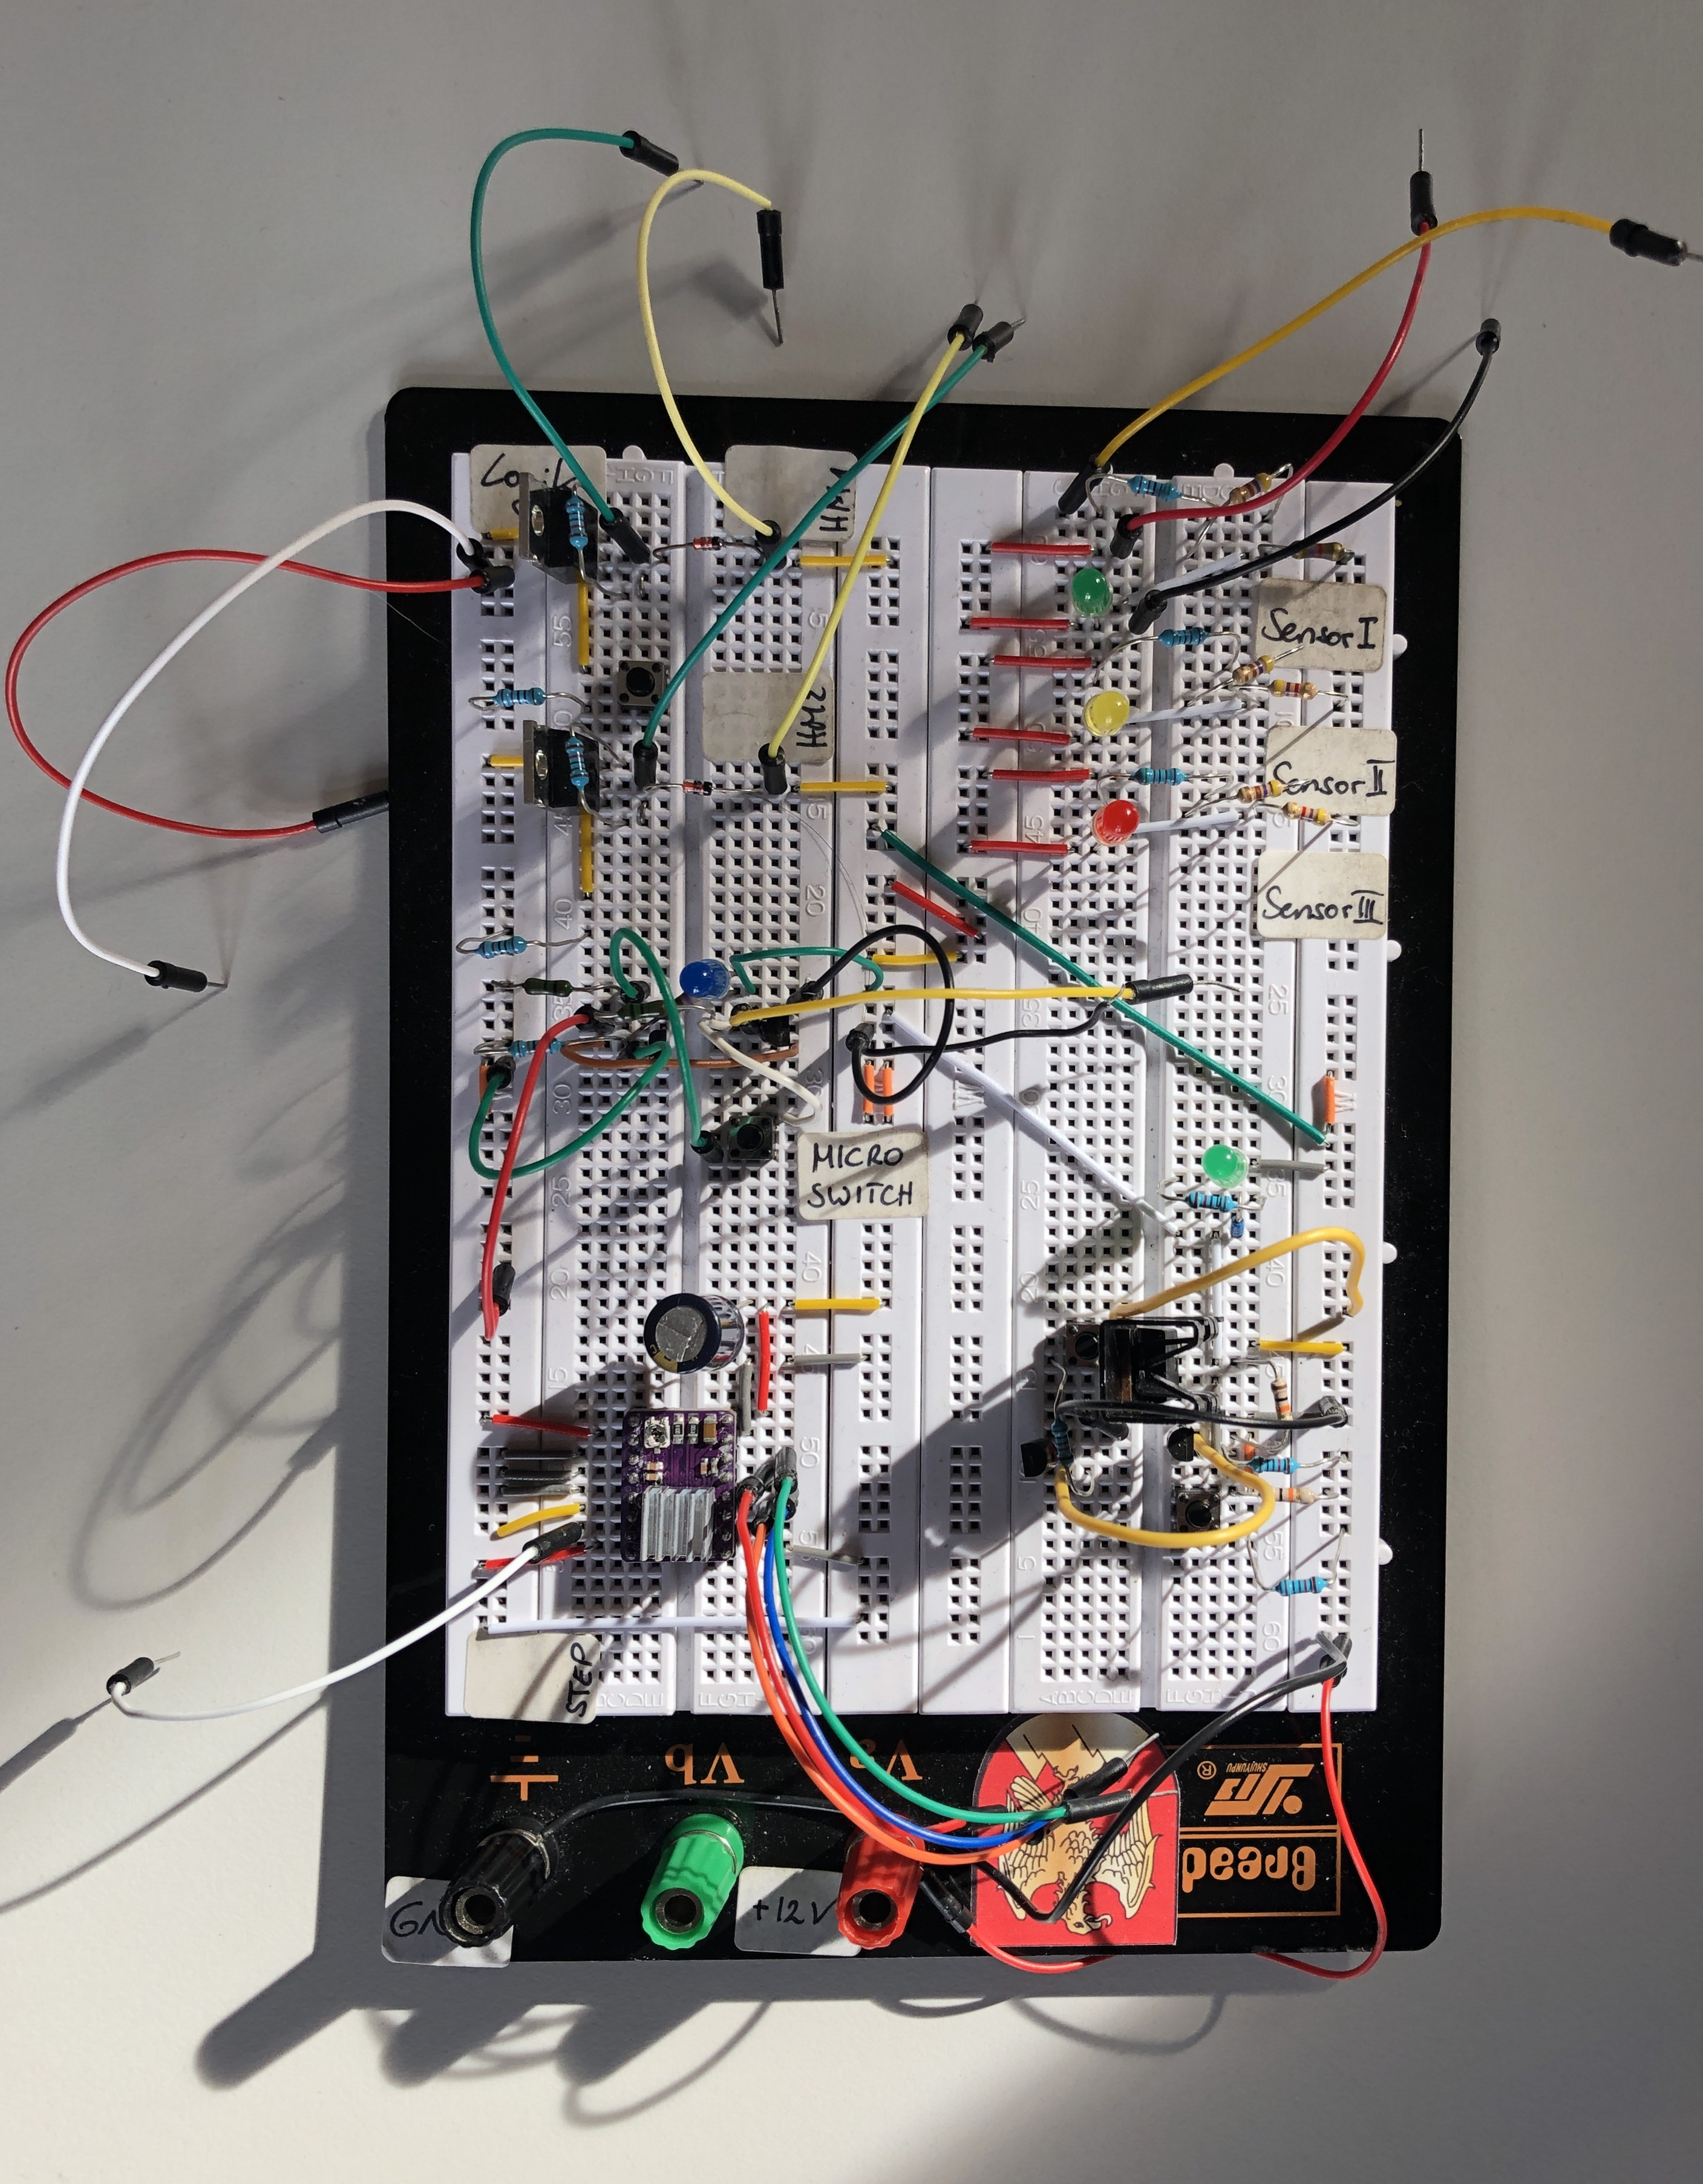
\includegraphics[scale=0.08]{fig/elektro/Steckbrett}
    \caption{Diverse Schaltungen in der Praxis}
\end{figure}

Sobald die Funktionstüchtigkeit einen praktischen Hintergrund angenommen hatte,
war es an der Zeit jegliche Bauteile für die Leiterplatte auszuwählen und zu dimensionieren.

%/\-/\-/\-/\-/\-/\-/\-/\-/\-/\-/\-/\-/\-/\-/\-/\-/\-/\-/\-/\-/\-/\-/\-/\-/\-/\-/\-/\-/\-/\-/\-/\-/\-/\-/\-/\-/\-/\-/\-/\-/\-/\-/\-/\-/\-/\-/\-/\-/\-/\-/\-/\-/\-/\-/\-/\-/\-/\-/\-/\

\newpage
\section{Auswahl der Bauteile}

\subsection{Auswahl der Transistoren}
\subsubsection{P-Kanal MOSFET}

Als P-Kanal MOSFET traf unsere Wahl auf den FDD6637.
Dieser bringt einen niedrigen Übergangswiderstand vom Drain zur Source mit sich.
Außerdem ist dieser dazu in der Lage, eine Spannung von maximal -35V zu schalten und gleichzeitig einen Strom von bis -55A treiben zu können.

\subsubsection{N-Kanal MOSFET}

Als N-Kanal MOSFET wählten wir den FDN337N aus, welcher in der Lage ist, Ströme von bis zu 2.2A treiben zu können.
Außerdem ist es diesem möglich, Drain-Source-Spannungen von bis zu 30V zu schalten, was für unsere Anwendung weitaus genügt.
Hinzu kommt noch die wesentliche Tatsache, dass dieser eine niedrige Gate Treshold Voltage von nur max.1V mit sich bringt.

\subsection{Auswahl der Gleichspannungswandler-Peripherie}

\subsubsection{Spule}
Um eine geeignete Spule für den Step-Down Wandler auszuwählen, wurde auf dessen Datenblatt zurückgegriffen.
Über die uns verwendete Eingangsspannung des Gleichspannungswandlers und den maximal fließenden Strom von 2A
traf unsere Entscheidung über eine Tabelle jener technischen Dokumentation auf eine Spule mit einem Wert von 100µH .
Über die Bedingung einen derartig hohen Strom treiben zu können, fiel unsere Wahl auf die DR127-101-R,
welche die Eigenschaften eines maximalen Gleichspannungsstroms von 3.64A, einen hohen Wirkungsgrad, magnetische Geschirmtheit und einem SMD-Gehäuse mit sich bringt.

\subsubsection{Schottky-Diode}
Bei der Wahl einer passenden Schottky-Diode wurde ebenfalls auf die technische Dokumentation des Gleichspannungswandlers zurückgegriffen.
Als günstige Lösung wurde die MBRD340 gewählt, da diese einen maxmimalen Strom von 3A standhalten kann und für Spannungen von bis zu 40V geeignet ist.

\subsection{Auswahl der Gleichrichter-Dioden}

Als diese Dioden selektierten wir die RR264M, welche sowohl einen Strom von 1A treiben kann, was wichtig für die Implemntierung an den induktiven Last ist.
Zusätzlich besitzt sie die Eigenschaft, einen Spannungsabfall von 0.7V bei einem Strom von 0.01A bei 25°C zu verursachen.
Dies ist essenziell für die Implementierung an jenen Spannungspegelüberwachungspunkten.

\subsection{Auswahl der Schottky-Dioden}

Als Schottky-Diode wählten wir die MBR130, welche die Maximalwerte von 1A und 30V mit sich bringt.
Außerdem ist anzuführen, dass ein wesentliches Attribut der an ihr niedriger, abfallender Spannungsabfall von nur 0.25V bei 25°C und 0.1A ist.
Bei 1A und 25°C beträgt der Spannungsabfall 0.35V .
Die Eigenschaften des niedrigen Spannungsabfalls in Anbetracht der UNLATCH-Schaltung und der Beschaltung des USB-UART-Converters befürworteten ihren Einsatz.

\subsection{Auswahl der Zener-Diode}

Als Zener-Diode selektierten wir die BZX84-C8V2, welche alle gewünschten Eigenschaften und eine Zenerspannung von 8.2V mit sich bringt.

\subsection{Auswahl sonstiger Bauelemente}

Bei den Bauformen jener Kondensatoren, dessen Wert 100nF oder 22pF beträgt, und aller Leuchtdioden und Widerstände wurde auf 0805er Chips zurückgegriffen,
da sich diese bereits in unserem Besiz befanden und diese eine platzsparende, und dennoch einfach zu lötende Lösung bereitstellten.
Bei der Auswahl der Kondensatoren im µF-Bereich wurde auf SMD-Elektrolytkondensatoren mit einem Diameter von 6 bis 8mm zurückgegriffen.

%/\-/\-/\-/\-/\-/\-/\-/\-/\-/\-/\-/\-/\-/\-/\-/\-/\-/\-/\-/\-/\-/\-/\-/\-/\-/\-/\-/\-/\-/\-/\-/\-/\-/\-/\-/\-/\-/\-/\-/\-/\-/\-/\-/\-/\-/\-/\-/\-/\-/\-/\-/\-/\-/\-/\-/\-/\-/\-/\-/\

\newpage
\section{Leiterplattendesign}

Sogleich die Auswahl der Peripherie beendet war, war es an der Zeit ein Design für die geplante Platine in KiCad zu entwerfen.
Als Anforderungen stellten wir uns ein möglichst kompaktes, strukturiertes sowie übersichtliches Design zu erstellen.
Hierzu kamen noch spezifischere Anforderungen, da bei einem Fertigen der Leiterplatte in der schuleigenen Werkstätte nur eingeschränkte Fertigungsparameter gegeben sind.
Zu diesen zählen ein Mindestbohrdurchmesser bei Durchkontaktierungen von 0.6 mm sowie die Tatsache, eine Mindestleiterbahnbreite von 0.2 mm zu verwenden.
Außerdem dürfen keine Durchkontaktierungen unter Bauteilen platziert werden, da bei diesen jeweils ein Leiter per Hand eingelötet werden muss.
Nennswert ist zudem, dass nur maximal zweilagige Leiterplatten angefertigt werden können.

\subsection{Layoutdesign}

Beim Layoutdesign wurde darauf geachtet, keine THT und SMD Bauteile zu vermischen.
Somit wurden diese jeweils auf zwei verschiedenen Layern platziert. \\
Im Laufe der Diplomarbeit entstanden unzählig viele, verschiedene Layouts, welche die Gründe von ständig neu aufkommenden Ideen, Ausmerzung von Fehlerquellen und Simplifizierungen hatten.
Diese Faktoren machten das Designen eines optimalen Layouts zu einer langwierigen, aber lehrreichen Aufgabe.
Eine falsche Dimensionierung von Bauteilen und Baugruppen und Denkfehler, die das Fertigen erschweren würden waren hierbei die Hauptfaktoren. \\

Die Breite aller Leiterbahnen wurden auf den maximal fließenden Strom ausgelegt.
Um zu diesen Werten zu kommen, wurde ein Tool angewandt, welches sich in der KiCad Nutzerumgebung finden lässt.
Dieses wendet folgende Formel an: \\

\begin{equation}
    I = K \cdot dT^{0.44} \cdot (W \cdot H)^{0.725}
\end{equation}
wobei
\begin{itemize}
    \item I dem maximal fließenden Strom in Ampere,
    \item K 0.048 für externe oder 0.024 für interne Leiterbahnen,
    \item dT dem Temperaturanstieg über der Umgebungstemperatur in Grad Celsius,
    \item W der Leiterbahndicke in mils und
    \item H der Leiterbahnbreite in mils entspricht.
\end{itemize}

Die folgend zu findenden Abbildungen zeigen die Vorder- und Rückseite des fertigen Leiterplattenlayouts.

\subsection{Leiterplattenfertigung}

\subsubsection{Prototyping}

Bevor wir fester Überzeugung aller Funktionen sein konnten, stellten wir uns die Fertigung eines funktionierenden Prototypen als Aufgabe.
Dies hat die Vorteile, etwa im Platinenlayout falsch Gemachtes, bereits vor der finalen Version zu erkennen und auszumerzen.
Jener Prototyp wurde in der Werkstätte der HBTLA Kaindorf angefertigt. \\

\textbf{Als Fertigungsschritte sind folgende zu nennen:}

\begin{itemize}
\item Zuallererst ist das Layout der Kupfervorderseite und der Kupferückseite jeweils auf eine transparentes Papier mit den bestmöglichen Einstellungen zu drucken.
Für einen erfolgreichen Druck ist ein Spiegeln der Vorderseite der Platine ein Muss.
Folgend ist ein Spray zum Verdichten des Toners anzuwenden.
Aus den zwei Stücken Transparentpapier ist eine Tasche anzufertigen, sodass jegliche Bohrungen genau gegenüberliegen. \\

\item Zunächst ist die Leiterplatte mithilfe der angefertigten Tasche eine Minute lang in der Belichtungsmaschine unter Vakuuum zu belichten. \\

\item Die beleuchtete Leiterplatte ist anschließend eine Minute lang in ein Natriumhydroxid-Bad zu begeben, um sie zu entwickeln. \\

\item Folgend ist sie mit heißem Wasser abzuspülen und in ein Natriumpersulfat-Bad zu geben.
Die Zeitdauer des Verweilens variiert je nach Belastung des Ätzbades.
In unserem Fall ätzten wir die Leiterplatte 17 Minuten. \\

\item Anschließend ist die Leiterplatte mit heißem Wasser abzuspülen und mit Azeton zu reinigen. \\

\item Als nächsten Schritt ist sie für einige Minuten in ein Zinnbad zu legen. \\

\item Nun kann die Leiterplatte ein letztes Mal mit heißem Wasser gereinigt und mit Fluxclean gereinigt werden.

\item Letztendlich kann der exakte Zuschnitt und das Bohren durchgeführt werden. \\

\item Zuletzt kann das Anfertigen von Durchkontaktierungen sowie das Bestücken der Leiterplatte erfolgen.
\end{itemize}

%/\-/\-/\-/\-/\-/\-/\-/\-/\-/\-/\-/\-/\-/\-/\-/\-/\-/\-/\-/\-/\-/\-/\-/\-/\-/\-/\-/\-/\-/\-/\-/\-/\-/\-/\-/\-/\-/\-/\-/\-/\-/\-/\-/\-/\-/\-/\-/\-/\-/\-/\-/\-/\-/\-/\-/\-/\-/\-/\-/\

\newpage
\section{Resümee und Aussichten für die Zukunft}
\subsection{Reflexion der Arbeit}

\subsection{Verbesserungsmöglichkeiten}

Sollte man die Versorgung des Raspberry Pi's über die GPIO Pins vornehmen, ist ein Überspannungsschutz nicht gegeben.
Eine essenzeille Schutzmaßnahme, um den Raspberry Pi bei einer zugeführten Überspannung nicht zu beschädigen, wäre ein sogenannter zu implementierender Crowbar-Circuit.
Diese Art von Schaltung ermöglicht es, empfindliche Komponenten vor Überspannung zu schützen.

\begin{figure}[hpt]
    \centering
    \begin{circuitikz}[european, scale = 1.2]
        \draw (0,0) node[anchor=east] {-} to [short, o-*] (2,0);
        \draw (2,0) to [R,l=$R1$, *-*](2,2) to [/tikz/circuitikz/bipoles/length=1cm, zD-, l=$D1$,-*](2,4);
        \draw (2,2) to (3.5,2);
        \draw (4,4) to [/tikz/circuitikz/bipoles/length=1.1cm, Ty-, mirror, l=$D2$,*-](4,0.915) to [short,-*](4,0);
        \draw (2,4) to [short, -o](0,4)node[anchor=east]{+};
        \draw (2,4) to [short, -o](6,4)node[anchor=west]{+};
        \draw (3,0) to [short, -o](6,0)node[anchor=west]{-};
        \draw (3,0) to (2,0) node[rground]{};
        \draw (0,3.8) -- node[left] {$U_\mathrm{e}$}node[sloped,currarrow,pos=1] {}(0,0.2);
        \draw (6,3.8) -- node[right] {$U_\mathrm{Last}$}node[sloped,currarrow,pos=1] {}(6,0.2);
    \end{circuitikz}
    \caption{Crowbar Circuit}
\end{figure}

Bei einer zulässigen Versorgungsspannung von 5V gelangt die Zenerdiode nicht in einen leitenden Zustand und eine sichere Versorgung der dahinter liegenden Schaltung ist gegeben.
Sobald der Wert der Versorgungsspannung jenen nominalen Zenerspannungswert der Zenerdiode übersteigt, wird diese leitend.
Überschüssige Spannung fällt somit am Widerstand ab, wobei die am Widerstand abfallende Spannung der am Gate anliegenden Spannung gleichzusetzen ist.
Sollte diese Spannung die maximalen Gate-Triggerspannung übersteigen, zündet das Gate des Thyristors und er wird leitend.
Somit schließt der Thyristor die dahinter liegende Schaltung kurz und ein Schutz der sensiblen Komponenten ist gegeben. \\

Diese Schaltung konkret auf unsere Anwendung angewandt, wären die Komponenten wie folgt zu wählen:
\begin{itemize}
    \item R1 mit etwa 10kOhm
    \item D1 mit einer Zenerspannung von 4.3V
    \item D2 mit möglichst niedriger maximaler Gate-Triggerspannung, z.B.0.8V
\end{itemize}

%/\-/\-/\-/\-/\-/\-/\-/\-/\-/\-/\-/\-/\-/\-/\-/\-/\-/\-/\-/\-/\-/\-/\-/\-/\-/\-/\-/\-/\-/\-/\-/\-/\-/\-/\-/\-/\-/\-/\-/\-/\-/\-/\-/\-/\-/\-/\-/\-/\-/\-/\-/\-/\-/\-/\-/\-/\-/\-/\-/\